\newif\ifdraft\drafttrue
\newif\iflater\latertrue
\newif\ifnext\nexttrue
\newif\iflast\lastfalse

\newif\ifthemecolors\themecolorsfalse % colorize section 2?

% John's comments
%  https://docs.google.com/document/d/1Yt-TFaC_TPu9KqcPEg3z1la-GphyhA3u9FZ7fcvG3TI/edit#

%  GPG:
% https://www.nsf.gov/pubs/2023/nsf23524/nsf23524.htm

\documentclass{NSF}

\graphicspath{{figures/}}

\usepackage{url}
\usepackage{wrapfig}
\usepackage{tabularx}
\usepackage{datetime2}
\usepackage[final]{pdfpages}

\newcommand{\participant}[1]{{P#1}}

\usepackage{xcolor}
\definecolor{nord-night1}{HTML}{2e3440}
\definecolor{nord-night2}{HTML}{3b4252}
\definecolor{nord-night3}{HTML}{434c5e}
\definecolor{nord-night4}{HTML}{4c566a}
\definecolor{nord-snow1}{HTML}{d8dee9}
\definecolor{nord-snow2}{HTML}{e5e9f0}
\definecolor{nord-snow3}{HTML}{eceff4}
\definecolor{nord-frost1}{HTML}{8fbcbb}
\definecolor{nord-frost2}{HTML}{88c0d0}
\definecolor{nord-frost3}{HTML}{81a1c1}
\definecolor{nord-frost4}{HTML}{5579a5}
\definecolor{nord-red}{HTML}{b14853}
\definecolor{nord-orange}{HTML}{c76d52}
\definecolor{nord-yellow}{HTML}{ebcb8b}
\definecolor{nord-green}{HTML}{69894d}
\definecolor{nord-purple}{HTML}{815679}
\definecolor{nord-red1}{HTML}{cc7777}
\definecolor{nord-red4}{HTML}{994444}

\usepackage{listings}
\lstset{
  keepspaces=true,
  mathescape=true,
  frame=none,
  xleftmargin=10pt,
  stepnumber=1,
  belowcaptionskip=\bigskipamount,
  captionpos=b,
  % language=haskell,
  % breaklines=true,
  tabsize=2,
  emphstyle={\bf},
  commentstyle=\it\color{cb-blue},
  stringstyle=\mdseries\ttfamily,
  showspaces=false,
  keywordstyle=\bfseries\ttfamily,
  deletekeywords={split},
  columns=flexible,
  basicstyle=\ttfamily,
  showstringspaces=false,
  morecomment=[l]--,
  moredelim=**[is][\color{nord-green}]{@}{@},
  moredelim=**[is][\color{nord-frost4}]{~}{~},
  moredelim=**[is][\color{nord-orange}]{£}{£},
  literate={cP}{{$\mathcal{P}$}}1
  {cG}{{$\mathcal{G}$}}1
  {cGhat}{{$\overline{\mathcal{G}}$}}1
  {cC}{{$\mathcal{R}$}}1
  {cL}{{$\mathcal{L}$}}1
  {fmap}{{$\fmap$}}3
  {[[}{{$\llbracket$}}1 % chktex 9
  {]]}{{$\rrbracket$}}1 % chktex 9
  % {->}{{$\rightarrow$}}2
  % {return}{{$\return$}}6
  % {pick}{{$\pick$}}4
  % {void}{{$\void$}}4
  % {do}{{$\textbf{do}$}}2
  % {>>=}{{$\bind$}}2
  % {<-}{{$\leftarrow$}}2
  % {\\}{{$\lambda$}}1
  % {==>}{{$\implies$}}3
  % {=>}{{$\Rightarrow$}}2
  % {<|>}{{$\langle | \rangle$}}2
}

\newcommand{\thread}[1]{\textbf{\emph{#1}}}
\newcommand{\tyche}{{\sc Tyche}}
\newcommand{\citet}[1]{\cite{#1}\todo{fixme}}
\newcommand{\citeauthor}[1]{\cite{#1}\todo{fixme}}

% Macros pilfered from HATRA submission
\definecolor{dkred}{rgb}{0.7,0,0}
\definecolor{dkpurple}{HTML}{4e02eb}
\definecolor{dkgreen}{HTML}{006329}
\definecolor{teal}{HTML}{007982}
\definecolor{string}{HTML}{02782d}
\definecolor{Fuchsia}{HTML}{8C368C}
\definecolor{quoteblue}{HTML}{2264b4}
\definecolor{gray}{HTML}{BBBBBB}
\definecolor{darkgray}{HTML}{555555}

\newcommand{\comm}[3]{\ifdraft\textcolor{#1}{[#2: #3]}\fi}
\newcommand{\cn}{\ifdraft{\color{blue} [CITE]}\fi}
\newcommand{\bcp}[1]{\comm{dkpurple}{BCP}{#1}}
\newcommand{\rjmh}[1]{\comm{nord-green}{RJMH}{#1}}
\newcommand{\rjmhlater}[1]{\iflater\comm{nord-green}{RJMH}{#1}\fi}
\newcommand{\bcplater}[1]{\iflater\comm{dkpurple}{BCP}{#1}\fi}
\newcommand{\bcplast}[1]{\iflast\comm{dkpurple}{BCP}{#1}\fi}
\newcommand{\bcpread}[1]{\iflater\comm{red}{BCP}{Read #1}\fi}
\newcommand{\hg}[1]{\comm{dkred}{HG}{#1}}
\newcommand{\harry}[1]{\hg{#1}}
\newcommand{\jwc}[1]{\comm{dkgreen}{JC}{#1}}
\newcommand{\amh}[1]{\comm{teal}{AH}{#1}}
\newcommand{\comment}[1]{{\em #1}}
\newcommand{\todo}[1]{\ifdraft {\color{nord-red} TODO: #1} \fi}
\newcommand{\todolater}[1]{\iflater\ifdraft {\color{nord-red} TODO: #1} \fi\fi}
\newcommand{\todolast}[1]{\iflast\ifdraft {\color{nord-red} TODO: #1} \fi\fi}
\newcommand{\writeme}[1]{{\color{blue} #1}}
\newcommand{\rewrite}[1]{{\ifdraft\color{dkred}\fi #1}}
% \newcommand{\pagebudget}[1]{(#1 pages)}
\newcommand{\pagebudget}[1]{}
\newcommand{\underconstruction}[1]{{\color{nord-red} Under construction: #1}}

\newcommand{\forreaders}[1]{}
\newcommand{\discuss}[1]{{\color{purple}\bf High priority: #1}}

\usepackage{ulem}\normalem
\newcommand{\proposecut}[1]{\iflater\ifdraft{\color{gray} \sout{#1}}\fi\fi}
\newcommand{\proposechange}[2]{\ifdraft{\color{gray} \sout{#1}
    $\rightarrow$ #2}\else #2\fi}

\newcommand{\jsquote}[2]{%
  \begin{center}
  {\color{darkgray}
    \fbox{
      \color{black}
      \begin{minipage}{0.87\linewidth}
        ``#2''  \hfill --Participant #1
        \end{minipage}
        }
    }
  \end{center}
}

\usepackage[inline]{enumitem}
\usepackage{anyfontsize}
\newcommand{\headerfont}{\fontsize{11}{13}\selectfont\bf}

%%%%%%%%%%%%%%%%%%%%%%%%%%%%%%%%%%%%%%%%%%%%%%%%%%%%%%%%%%%%%%%%%%%%%%%%%%%
%%%%%%%%%%%%%%%%%%%%%%%%%%%%%%%%%%%%%%%%%%%%%%%%%%%%%%%%%%%%%%%%%%%%%%%%%%%
%%%%%%%%%%%%%%%%%%%%%%%%%%%%%%%%%%%%%%%%%%%%%%%%%%%%%%%%%%%%%%%%%%%%%%%%%%%

\usepackage{ifthen}
\usepackage{pgfgantt}

\newcommand{\publicationtarget}[1]{\smallskip{\em Publication target:} #1.}
\newcommand{\discussiontarget}[1]{\smallskip{\em Presentation target:} #1.}
% \newcommand{\publicationtarget}[1]{\smallbreak\noindent We plan to publish this
% work at #1.}
% \newcommand{\discussiontarget}[1]{\smallbreak\noindent We plan to present this
% work at #1.}

\newwrite\workplanfile
\immediate\openout\workplanfile=\jobname.workplan

\newcommand{\techtransfercolor}{nord-purple}
\newcommand{\educationcolor}{nord-green}
\newcommand{\pltheorycolor}{nord-frost1}
\newcommand{\plpracticecolor}{nord-frost4}
\newcommand{\hcitheorycolor}{nord-red1}
\newcommand{\hcipracticecolor}{nord-red4}
\newcommand{\piercecolor}{nord-red4}
\newcommand{\headcolor}{nord-frost4}
\newcommand{\bothcolor}{nord-purple}
\newcommand{\phdonecolor}{nord-frost1}
\newcommand{\phdtwocolor}{nord-frost4}
\newcommand{\phdthreecolor}{nord-red1}
\newcommand{\phdfourcolor}{nord-red4}
\newcommand{\engineercolor}{nord-green}
\newcommand{\facultycolor}{nord-yellow}

\newcommand{\COLOROF}[1]{%
  \ifthenelse{\equal{#1}{Tech Transfer}}
  {\edef\FOO{\techtransfercolor}}
  {\ifthenelse{\equal{#1}{Education}}
  {\edef\FOO{\educationcolor}}
  {\ifthenelse{\equal{#1}{PL Theory}}
  {\edef\FOO{\pltheorycolor}}
  {\ifthenelse{\equal{#1}{PL Practice}}
  {\edef\FOO{\plpracticecolor}}
  {\ifthenelse{\equal{#1}{HCI Theory}}
  {\edef\FOO{\hcitheorycolor}}
  {\ifthenelse{\equal{#1}{HCI Practice}}
  {\edef\FOO{\hcipracticecolor}}
  {\ifthenelse{\equal{#1}{Head}}
  {\edef\FOO{\headcolor}}
  {\ifthenelse{\equal{#1}{Pierce}}
  {\edef\FOO{\piercecolor}}
  {\ifthenelse{\equal{#1}{Both}}
  {\edef\FOO{\bothcolor}}
  {\ifthenelse{\equal{#1}{PhD 1}}
  {\edef\FOO{\phdonecolor}}
  {\ifthenelse{\equal{#1}{PhD 2}}
  {\edef\FOO{\phdtwocolor}}
  {\ifthenelse{\equal{#1}{PhD 3}}
  {\edef\FOO{\phdthreecolor}}
  {\ifthenelse{\equal{#1}{PhD 4}}
  {\edef\FOO{\phdfourcolor}}
  {\ifthenelse{\equal{#1}{Engineer}}
  {\edef\FOO{\engineercolor}}
  {\ifthenelse{\equal{#1}{Faculty}}
  {\edef\FOO{\facultycolor}}
  {\edef\FOO{white}}
}}}}}}}}}}}}}}}
\newcommand{\colorkey}[1]{%
  %\COLOROF{#1}%
  %\FOO = #1%
}

\newcommand{\SIMPLESECTION}[2]{\section{#1}\label{#2}}
\newcommand{\SECTION}[3]{%
  \SIMPLESECTION{#1: #2}{#3}%
  \immediate\write\workplanfile{\string\ganttsection{#1}\string\relax}
}
\newcommand{\sectionstar}[1]{\subsection*{#1}}
% \newcommand{\subsectionstar}[1]{\paragraph*{#1}}
\newcommand{\subsectionstar}[1]{
  \medskip \noindent {\headerfont #1.}}
% \newcommand{\subsectionstar}[1]{\subsubsection*{#1}}
\newcommand{\SUBSECTION}[8]{%
  \refstepcounter{subsection}%
  \bigskip \noindent {\headerfont \thesubsection\ \ #1.}%
  % \subsection{#1}
  \label{#2}%
  \COLOROF{#6}%
  % \ifthenelse{\equal{#5}{Benjamin}}{%
  %   \edef\FOO{\benjamincolor}%
  % }{%
  % \ifthenelse{\equal{#5}{Andrew}}{%
  %   \edef\FOO{\andrewcolor}%
  % }{%
  % \ifthenelse{\equal{#5}{Both}}{%
  %   \edef\FOO{\bothcolor}%
  % }{%
  %   \edef\FOO{\othercolor}}%
  % }}%
  \immediate\write\workplanfile{%
    \string\tasksection{#1
        (\string\sectionref{#2})}{#2}{#3}{#4}{\FOO}{#5}{#6}{#7}{#8}\string\relax}%
}
\newcommand{\tasksectiongantt}[9]{%
%  \ifthenelse{\equal{\currentganttsection}{Foundation}}%
  \ganttnewline
%    {\ganttnewline[grid]}
  \ganttbar
       [bar/.append
          style={fill=#5}]
%          style={fill=gray}]
       {\hbox to 3in{{\footnotesize {\bf \currentganttsection}
                     \hfill
                     #1}}}
       {#3}{#4}
  \gdef\currentganttsection{}
}
\newcommand{\sectionref}[1]{\S\ref{#1}}
\newcommand{\tasksection}{\tasksectiongantt}

\newcommand{\TASK}[4]{}
\newcommand{\TASKnotneeded}[4]{%
  \ifthenelse{\equal{#2}{#3}}{%
    \edef\FOO{year #2}%
  }{%
    \edef\FOO{years #2--#3}%
  }
  \smallskip {\it{Task: #1 (\FOO, #4).}}
  % \ifthenelse{\equal{#4}{Harry}}{%
  %   \edef\FOO{\harrycolor}%
  % }{%
  % \ifthenelse{\equal{#4}{Both}}{%
  %   \edef\FOO{\bothcolor}%
  % }{%
  %   \edef\FOO{\othercolor}}%
  % }%
  \immediate\write\workplanfile{%
    % \string\task{#1 (#4)}{#2}{#3}{\FOO}}%
    \string\task{#1 (#4)}{#2}{#3}}%
}
\newcommand{\task}[3]{
    {\ganttnewline}
  \ganttbar
       [bar/.append
          style={fill=white}]
       {\hbox to 3in{\hfill \footnotesize \it #1}}
       {#2}{#3}
}

\ganttset{bar height=.6}
%\ganttset{hgrid style/.style=black}
\newcommand{\ganttsection}[1]{%
  \gdef\currentganttsection{#1}%
  %  \\ \ganttbar[bar/.append style={draw=white}] {\bf\small #1}{2}{3}
  }
\gdef\currentganttsection{}

%%%%%%%%%%%%%%%%%%%%%%%%%

\newcommand{\tasksectionroles}[9]{%
%  \ifthenelse{\equal{\currentganttsection}{Foundation}}%
  \ifthenelse{\equal{\currentganttsection}{}}{}{{\bf \currentganttsection}\\}%
  \gdef\currentganttsection{}%
  \ \ \ #1 & #7 & #8 & #9 % & #6
  \\
}


% \makeatletter
% \newcommand{\SECTION}[1]{\section{#1}
%   \g@addto@macro\workplanitems{\ganttsection{#1}}
% }
% \makeatother
% \newcommand{\sectionstar}[1]{\subsection*{#1}}
% \newcommand{\subsectionstar}[1]{\paragraph*{#1}}
% % \newcommand{\subsectionstar}[1]{\subsubsection*{#1}}
% \newcommand{\SUBSECTION}[4]{%
%   \subsection{#1}
%   \label{#2}
%   \workplanitem{\task{#1}{#2}{#3}{#4} \\}
% }
% \newcommand{\sectionref}[1]{\S\ref{#1}}

% \usepackage{pgfgantt}
% \def\workplanitems{FOO}
% \makeatletter
% \def\workplanitem#1{%
%   \g@addto@macro\workplanitems{#1 }}
% \makeatother
% \ganttset{bar height=.6}
% \newcommand{\ganttsection}[1]{
%   \ganttbar[bar/.append style={draw=white}] {#1}{2}{3} \\}
% \newcommand{\task}[4]{
%   \ganttbar [bar/.append style={fill=gray}]
%     {\small #1 (\sectionref{#2})}{#3}{#4} \\ }

%%%%%%%%%%%%%%%%%%%%%%%%%%%%%%%%%%%%%%%%%%%%%%%%%%%%%%%%%%%%%%%%%%%%%%%%%%%
%%%%%%%%%%%%%%%%%%%%%%%%%%%%%%%%%%%%%%%%%%%%%%%%%%%%%%%%%%%%%%%%%%%%%%%%%%%
%%%%%%%%%%%%%%%%%%%%%%%%%%%%%%%%%%%%%%%%%%%%%%%%%%%%%%%%%%%%%%%%%%%%%%%%%%%

\begin{document}

% BCP: This is correct:
\title{CISE: Large: Property-Based Testing for the People}

\vfil
\begin{center}
{\huge \color{red} Draft of \DTMnow}
\end{center}
\vfil
% \bigskip\bigskip\bigskip\bigskip
% \todo{More title ideas:
%   \begin{itemize}
%   \item Property-Based Testing for the People
%   \item (what else?)
%   \end{itemize}
% }

% \title{Property-Based Testing for the Working Programmer}
% \tableofcontents % TODO Remove?
%  BCP - was not working for me, so I followed the instruction to
%  remove :-)
\newpage

% A. Cover Sheet
% A number of the boxes contained on the Cover Sheet are
% electronically pre-filled as part of the FastLane login process
% Complete the rest of your info there

% B. Project Summary
\newsection{B}
\section*{Project Summary}

\todo{``Overview'' needed?}
\subsubsection*{Overview}
Property-based testing (PBT) is an advanced software engineering
methodology where users write executable formal specifications of system
components
and an automated test harness checks these specifications against
many automatically generated inputs.  The bug-finding power of PBT
arises its ability both to work with rich specifications and
to exercise a wide range of system behaviors---both
expected and unexpected---with minimal user guidance.
%
From its roots in the Haskell QuickCheck library, PBT has become
the testing method of choice across much of the functional programming
community; it has also begun to make inroads into industrial practice
at companies such as Quviq, Galois, Stripe, and
Amazon. \forreaders{Any other big companies?  Notable open-source
  projects?}
%
The goal of this proposal is to accelerate this transition
by addressing key challenges in
present-day PBT tools.

What are these challenges?
A need-finding study of PBT at Jane
Street, a Wall Street firm with a focus on software
technology as a competitive advantage, found developers enthusiastic
about its {\em usefulness} but
sometimes frustrated with its {\em usability}.
%
Indeed, the study identified usability as an issue in both major aspects
of PBT methods---{\em specification} of properties and {\em
  generation} of random inputs. Moreover, it revealed challenges
around another aspect of PBT that has so far received less attention from
researchers: how programmers can {\em validate} the
effectiveness of testing.

% At the level of {\em specification}, developers wished for better
% support for expressing common requirements such as ``this
% high-performance implementation of a service must behave exactly the
% same as that reference model'' and for articulating properties of
% poorly modularized code.
% %
% Concerning the other main component of PBT, the {\em generation} of
% random test cases, \todo{...}
% %
% Developers also need better {\em validation} tools for checking
% that their testing is actually effective.\todo{blah}
% %
% Finally, better {\em education} of potential PBT users is critically
% required.

% \amh{How about the following framing? In this project, we define a practice of
% usable property-based testing, and conduct foundational research in PL and HCI
% to bring about this practice. We define usable property based-testing as having
% two main components. First, providing visibility into what can be extremely
% complex test outcomes. Second, supporting the efficient expression of
% tests.\ldots{} And then we can jump into talking about the challenges that we
% plan to solve in specification, generation, validation, and education.}.
% %
% At the level of {\em specification}, developers wished for better
% support for expressing common requirements such as ``this
% high-performance implementation of a service must behave exactly the
% same as that reference model'' and for articulating properties of
% poorly modularized code.
% %
% Concerning the other main component of PBT, the {\em generation} of
% random test cases, \todo{...}
% %
% Developers also need better {\em validation} tools for checking
% that their testing is actually effective.\todo{blah}
% %
% Finally, better {\em education} of potential PBT users is critically
% required.

%  and ``shrinking'' of failing
% tests to minimal counterexamples,

To make PBT more usable, two largely disjoint
research areas must be
brought to bear.  PBT itself is grounded in domain-specific languages
and formal methods---traditional topics in the field of Programming Languages.
Usability, on the other hand, is the domain of Human-Computer Interaction.
%
This four-year project will combine insights, methods, and tools from
PL and HCI to advance the usability of PBT along all three of its
axes---specification, generation, and validation\iflater\todo{We may
  need to reorder these, depending on what happens with the global
  structure.}\fi---and bring it to a
broad community of software developers.

\smallskip

\noindent{\bf Keywords:} Programming languages; human-computer
interaction; property-based testing; usability.

\subsubsection*{Intellectual Merit}
The project will advance knowledge along four interconnected axes.
%
First, it will establish a firm {\bf\em foundation} for HCI-informed
research on PBT, supplementing past and ongoing user studies with
broader surveys of PBT across the software industry and real-time
observations of developers interacting with PBT.
%
Second, it will offer developers more usable {\bf\em specification} tools,
including a language for stating temporal properties over internal
program states and automation for model-based testing of
modular abstractions.
%
Third, it will explore a novel abstraction for random input {\bf\em
  generation} that enables a range of use cases---generating inputs
satisfying validity conditions, mutating inputs to explore the space
of similar inputs, and manually or automatically tuning a random
generator's distribution based on examples or code coverage.
%
And fourth, it will develop new interactive tools for rapid {\bf\em
  validation} of the effectiveness of testing, for helping programmers pin
down the causes of failures, and for visualizing generated data
distributions to support comprehension and tuning.

%  (1) deploy tools from HCI to better
% understand the challenges to wider adoption of PBT, (2) combine PL and
% HCI methods to build solutions, and (3) develop educational materials
% to make PBT concepts and tools accessible to a broad community of
% university students and industrial developers.

\subsubsection*{Broader Impacts}
A fifth thread of activity, coordinated with the rest and integral to the
project's aims, will be advance {\bf\em education} in PBT in both universities and industry. We will
develop materials for teaching industry programmers how to identify
high-leverage situations for using PBT, curricula for teaching mature
and powerful PBT practices to undergraduate students, and tooling to help
PBT beginners write their first properties.
%
A general-audience article on PBT for CACM will also help broaden the
reach of PBT.

Work on the project will include and elevate undergraduate
researchers, including some from diverse backgrounds that will be
funded through a new NSF-REU. These undergraduates will work
closely with the two PIs and four Ph.D.{} students in an interconnected and supportive
research environment.

The ultimate goal, through education, publications, and open-source
tools, is to make property-based testing a standard tool on every
software developer's testing toolbelt.  Better testing, in turn, will
lead to software systems of every sort that are less expensive, more
robust, and more reliable.


% The statement on broader impacts should describe the potential of the proposed activity to benefit society and contribute to the achievement of specific, desired societal outcomes.


% C. Table of Contents
% A Table of Contents is automatically generated for the proposal by FastLane

% D. Project Description
\newpage\newsection{D}
\section{Project Description \pagebudget{.5}}

\comment{Meta comment: I think a lot of the technical content here can come from my thesis proposal. It has all of the technical projects other than the benchmarking project (which BCP should be able to write about — or maybe ask for Jessica’s help?) and it also has the background and related work. It may be useful to go to the individual papers for some deeper details, but I’d be surprised.}

\todo{Harry proposal page 4 and 6.5-8}

\todo{
[MODEL AFTER THESIS INTRO / CONCLUSION]
\begin{itemize}
   \item High level: Advance the theory and practice of PBT, making it more valuable to a wider range of software engineers
   \item PBT is great
\begin{itemize}
      \item For people who like formal methods, it’s a way to write a formal spec and check it without doing full verification
      \item Even for people who don’t, it’s been extremely effective finding bugs in practice
         \item Cite…
      \item (?) And people really like it (maybe pull quotes from preliminary study)
\end{itemize}
   \item But there is still room for PBT to grow (maybe stats, feel free to refine this argument more)
   \item We want to advance the theory and practice of PBT so it is more valuable to SEs
\end{itemize}
}

\subsection{Background and Related Work \pagebudget{1.5}}

\subsubsectionstar{PIs' Prior Qualifications}

\subsection{Extending the Foundation \pagebudget{3}}

\todo{
\begin{itemize}
   \item Story
\begin{itemize}
      \item The research community has identified that random generation (and in particular, the valid generation problem)[b] causes problems for testers
      \item This shows up in prior work, and also in realistic examples (e.g., the fuzzing community really cares about this!)
      \item We’ve already done some work to explore new abstractions for random generation (free generators) and we have more that we want to try (reflective generators)
      \item In addition, the PBT community is missing tools to empirically evaluate generation strategies
      \item And the PBT literature is also woefully disconnected from the fuzzing literature, where they have their own partial solutions to this problem
\end{itemize}
   \item Prior Work - Free generators [CHAPTER 1[c] OF THESIS PROPOSAL is a
   source, but it's way too long -- we need to write a compact precis of the
   crucial points]
   (perhaps also some other prior things)
   \item Planned Work - Reflective generators [CHAPTER 2 OF THESIS PROPOSAL]   (needs new work on evaluation; maybe rests on benchmarking infrastructure; validity-preserving mutation scheme needs to be evaluated by real implementation and measurement)
   \item Planned Work - Empirical Evaluation Playground [JESSICA OR BENJAMIN WRITE] (can ultimately be used for Benchmarking; in the short term, it’s a playground for individual PBT efforts to see how they are doing)
   \item Speculative Work - Add PBT incrementally to a fuzzing system [CHAPTER 3 OF THESIS PROPOSAL](follows directly from the free and reflective generators work)
\end{itemize}
}

\subsection{Finding out what working programmers need \pagebudget{3}}

\todo{
\begin{itemize}
   \item Story
\begin{itemize}
      \item The projects above follow the lead of prior work, solving problems that have already been identified, but we have no reason to believe that those problems are exhaustive
      \item Indeed, there may be high-leverage opportunities to improve PBT that have nothing to do with the valid generation problem
      \item We’re in the process of uncovering “unknown unknowns” by talking to PBT users about their experiences - we’ve already done a preliminary study, and we plan on talking to Jane Street developers for a full-scale study
      \item We’re not sure what we should do after that, but the preliminary study gave us some ideas
\begin{itemize}
         \item We can obviously keep talking to users (via surveys or observations)
         \item We also identified that there are likely workflow improvements that could help PBT fit into a developer’s environment better (and user-centered design opportunities there)
         \item We may even find interesting PBT opportunities at Jane Street that will give us a hands-on opportunity to solve problems that real developers are actively dealing with
\end{itemize}
\end{itemize}
   \item Prior Work - Pilot study [CHAPTER 4 OF THESIS PROPOSAL / HATRA]
   \item Planned Work - Jane Street Study [CHAPTER 4 OF THESIS PROPOSAL / HATRA]
\end{itemize}
}


Part 1 of the ``unknown unknowns''.
Jane Street study, preliminary study, observations, surveys.

In this aim, we plan to set course for research in PBT, both broadly and for the
future directions of our group. We will conduct a series of formative studies,
each addressing one of three main goals:

\subsubsectionstar{Understanding Challenges to Using PBT Tools}

The first step is to conduct qualitative interviews to understand the challenges
that programmers face when using PBT tools.

Here I will elaborate on the design of the Jane Street study.

\subsubsectionstar{Characterizing the Potential Reach for PBT Tools}

We will conduct a survey with the purpose of understanding the impact that
improved PBT tools could have in industry, if major usability issues were
addressed. We see this survey as crucial in understanding the amount of
resources that should be devoted to PBT research. Furthermore, this
questionnaire will help shed light into which of the usability challenges from
the interview study, if addressed, are most likely to impact a broad set of
current and prospective users of PBT tools.

\subsubsectionstar{Understanding the Structure of PBT Tasks in Detail}

The next step is to more deeply characterize the obstacles faced with specific
tools and tasks through close observation. We anticipate conducting observations
of participants formulating properties and creating generators, as we expect
that close observation of developers performing these tasks will yield yet
additional detail about ways that developers are supported and not supported by
the tools they use today to a level of depth we will not achieve with the
interviews.

\subsection{Exploiting the Foundations to Build Powerful, Interactive PBT Tools \pagebudget{3}}

Upon the advanced technical foundation from Aim 1 and the refined understanding
of programmers' needs from Aim 2, our final aim (Aim 3) will focus on the
development of programmer-facing tools that allow them to leverage properties in
testing their code more efficiently and effectively.

While the specific focus of our tool design and research efforts will be
continually refined on the basis of what we learn from Aim 2, below we detail
several directions that we expect to lead to the design of tools that are both
innovative within the research community, as well as potentially impactful,
drawing on the lessons learned from the preliminary need-finding research we
have done to date as well as our own intuitions, and as critical users and
engaged members of the communities for these tools.

\todo{Discuss:

\begin{itemize}

% \item Some of the tools we propose in this section may depend on a technical
% background we do not have on this team. For instance, property generation.
% Should we be keeping the scope of the proposed work to those where we as a team
% have expertise in the backend technologies? After discussing with BCP, we need
% not limit ourselves to areas where we are at present the leading experts. Let's
% draft the descriptions, see the ones we are excited about, wave away some
% of the details that we have not yet educated ourselves, and go from there.

\item We should ask Jane Street for a letter of support indicating their
willingness to collaborate on the need-finding activities.

\end{itemize}
}

\subsubsectionstar{Interactive property specification}

Developers in the preliminary interview study indicated that while they knew their software would benefit from property-based testing, sometimes they had difficulty imagining which properties to test. One area that could benefit from innovation in PBT tools is in designing tools that help programmers imagine properties in situations like these.

To date, research has shown the potential for automated tools to extract invariants describing a program's behavior\cite{ammons2002mining,le2018deep,claessen2010quickspec}. However, the integration of such tools into developer workflows is non-trivial. We posit that a usable tool that can help with imagining properties would need the following features:

\textit{Readable code generation}. While prior techniques have succeeded in generating invariants, we expect that users of PBT systems would benefit from having properties generated in the language of their property-based testing tools. Furthermore, there are some variants about systems that may be so complex that they require significant comprehension time for users (i.e., those involving a large number of clauses). In such cases, a tool may way to generate simpler variants of properties first, and allow developers to refine them on their own.

\textit{Generating important properties}. Non-trivial programs can be described by an overwhelmingly large number of properties, many of which describe only incidental aspects of the program's behavior that do not need to be tested. How can tools produce those properties that developers would want to have tested? We believe that this is a problem that can be best solved with a mixed-initiative approach~\cite{allen1999mixed}---that is, judiciously incorporating both developer input and automation. Developer could guide a specification mining tool to extracting relevant properties through input mechanisms such as (1) identifying regions of code that are likely to lead to an adverse behavior such as an exception or a logical error; (2) providing unit test cases that test a special case of a generalized property; and (3) indicating aspects of interest on input and output data during exploration in a debugging REPL.

\textit{Property refinement}. Tools could help a developer refine generated properties. If a generated property is too relaxed, the tool could request that developer provides a counterexample that should trigger a failure, and then regenerate the property. If a generated property is too strict, a tool could allow a programmer to mark a counterexample that was generated by the PBT tool as spurious, i.e., not indicating an actual failure of the program. In each of these cases, the property generator may have generate multiple properties for a developer to review, each of which may satisfy the refinements that a developer has provided.

\textit{Plan of work}: Incorporating known, widely-used specification mining tools such as QuickSpec~\cite{claessen2010quickspec}\ldots{}

% One challenge identified by software developers we have spoken with is that it can be difficult to come up with a property to test with property-based testing tools. Perhaps tools could help programmers come up with, and express, properties that they wish to be tested. To design such tools, we will adapt techniques from the specification mining literature to generate candidate properties (e.g.,~) and interfaces that help programmers select from, and refine, generated properties.
% 
% A first step will be to generate candidate properties. These will be generated using specification mining techniques. Specifications will need to be mapped from an abstract representation of the property to an expression of that property in the programming language, such as Hypothesis' property specification language. A major challenge is that a specification mining technique will produce many spurious properties which do not describe aspects of the program that the programmer wishes to test. Affordances will be added to the programming environment to allow a program to select subsets of code that manipulate properties of interest; and to generalize from behaviors that are implied by individual unit tests, or observations made during debugging, to greatly limit the space of generated properties.
% 
% A second step will be to assist in the refinement of properties. In some cases, generated properties will be too broad; for instance, . if the testing tools yield a counterexample, the counterexample may be an indicator that a property is insufficiently strict, rather than an indication that the program is incorrect. @Andrew, continue from here\ldots{}
% 
% Motivation: Informants struggled to figure out what to test. informants had an intuitive idea of what “right” and “wrong” was. Perhaps they could have been helped with a tool that refined that expectation into something that was formal.
% 
% Plan of work: A first step in this process might be a tool that refines a wrong specification that has some counterexamples into a clean, correct specification. When a counterexample is encountered, you can fix the program if it represents a bug, or you will have to refine a property if the property was not written correctly.
% Alternatively, a greenfield specification maker might depend on a machine learning backend. We need to know more about how this works. Perhaps speak to Mayur about unit test generation. The tool design would focus on coming up with usable property specifications, and potential some user input (e.g., pointing to parts of programs that should be involved in property creation). Could specifications be provided as natural language? QuickSpec works okay for Haskell using static analysis to determine invariants. We would need someone with ML or program synthesis background to work on this project.
% 
% Example: For a serialization / deserialization pair of functions, testing that the serialized deserialized string is the same version as the original string; the refinement is to exclude Unicode strings, which do not have to be supported by serialization functions.

\subsubsectionstar{Visualizing and tuning data distributions}

% (this topic is what Joe is most excited about)

% For visualizing data distributions...

Plan of work: easily computable summary statistics; as well as user-defined metrics for understanding what you care the most about from the distribution. Seeing what the “average” data structure is that is getting generated. For multimodal data, what are the different modes of data. The set of data types to be handled in PBT are: algebraic data types, lists, trees (this would also cover programs). Joe thinks we already have good visualizations for numbers, booleans, and strings; it is compositional data types that we lack good visualizations for. People need to (1) see representative examples (2) understand spread (3) indicate areas of the space that should not be explored.

% For tuning data distributions...

Plan of work: indicating areas of the distribution that should not be generated.

Example: writing a generator of programs (for instance, to test out a compiler). You want lots of different programs that make sense in different ways. You want large ones, small ones, ones that use variables in coherent ways, ones that don’t overuse certain constructs, ones that use a variety of different language features. You want the generated programs to be representative of those that people might write. You also want some weird programs to catch the edge cases, but you don’t want all weird programs. (How big, how deep, how wide of programs?). Also, for trees, one might want to specify heights and breadths of the tree.

\subsubsectionstar{Debugging support for understanding counterexamples}

Once a PBT tool generates a counterexample of where a property fails, a programmer will need to understand what in an input caused the program to fail. This task can be rather challenging because generated inputs can be complex, deep data structures \todo{Do we have a reference that implies the complexity of generated counterexamples?}. Methods for making it clearer why a counterexample fails could be to generate additional inputs that are very close to the counterexample that are actually correct, to run the program up to the point where the traces of the programs begin to diverge, and then to drop a programmer into a debugging environment where they can query the state of the program and step through the remainder of the execution. PI Head has prior work designing debugging tools that help programmers understand trace divergences in an educational setting~\cite{suzuki2017tracediff}.

\subsubsectionstar{Reconciling generator API design with imperative language idioms}

Motivation: How do you design a generator DSL in an imperative language? A generator uses higher-level functions in a way that might be confusing to people who used Python.  (e.g., passing a generator of numbers to a generator of lists to get randomized lists of numbers). Is there a way of designing APIs for generators that can make the composition of these types of generators easier to reason about and express for some programmers?

(Joe says the DSLs are well-designed, but the code is hard to debug. How do you write a generator that works really well, that has a good data distribution and finds bugs? See below.)

Plan of work. Not sure. This might require some discussions with more uses of Hypothesis-like libraries.

Next steps—get examples of sloppily-expressed PBtests in Python and then think through how they would be written more clearly.

\subsubsectionstar{Integration with continuous integration workflows}

\todo{Section 6.2 of Harry's thesis proposal.}

\subsubsectionstar{Tailoring PBT for financial systems}

I am not sure what should go here. I am a bit wary of focusing specifically on developing tools for financial systems if the focus of this grant proposal is to make PBT tools more broadly useful.

\subsection{Education \pagebudget{1}}

\subsection{Plan of Work \pagebudget{.5}}

\subsection{Broader Impacts \pagebudget{.5}}
The Project Description must contain, as a separate section within the narrative, a section labeled ``Broader
Impacts of the Proposed Work". This section should provide a discussion of the broader impacts of the proposed
activities. Broader impacts may be accomplished through the research itself, through the activities that are
directly related to specific research projects, or through activities that are supported by, but are complementary to
the project. NSF values the advancement of scientific knowledge and activities that contribute to the
achievement of societally relevant outcomes. Such outcomes include, but are not limited to: full
participation of women, persons with disabilities, and underrepresented minorities in science, technology, engineering, and
mathematics (STEM); improved STEM education and educator development at any level; increased public
scientific literacy and public engagement with science and technology; improved well-being of individuals in
society; development of a diverse,globally competitive STEM workforce; increased partnerships between
academia, industry, and others; improved national security; increased economic competitiveness of the United
States; and enhanced infrastructure for research and education.

\subsection{Results from Prior NSF Support \pagebudget{.5}}
If any PI or co-PI identified on the project has received NSF funding (including any current
funding) in the past five years, in formation on the award(s) is required,
irrespective of whether the support was directly related to the proposal or not.
In cases where the PI or co-PI has received more than one award (excluding amendments),
they need only report on the one award most closely related to the proposal. Funding includes not just salary
support, but any funding awarded by NSF. The following information must be provided:\\

\noindent
\emph{\underline{Name of PI}}: NSF-Program (Award Number) ``Title of the Project'' (\$AMOUNT, PERIOD OF SUPPORT).
{\bf Publications:} List of publications resulting from the NSF award. A complete bibliographic citation for each
publication must be provided either in this section or in the References Cited section of the proposal); if
none, state: ``No publications were produced under this award.'' {\bf Research Products:} evidence of research products
and their availability, including, but not limited to: data, publications, samples, physical collections, software,
and models, as described in any Data Management Plan.

% \subsubsection{Proposed Study}
% The Project Description should provide a clear statement of the work to be undertaken and must include:
% objectives for the period of the proposed work and expected significance; relation to longer-term goals of the PI's
% project; and relation to the present state of knowledge in the field, to work in progress by the PI under other
% support and to work in progress elsewhere.
%
% The Project Description should outline the general plan of work, including the broad design of activities to be
% undertaken, and, where appropriate, provide a clear description of experimental methods and procedures.
% Proposers should address what they want to do, why they want to do it, how they plan to do it, how they will
% know if they succeed, and what benefits could accrue if the project is successful. The project activities may be
% based on previously established and/or innovative methods and approaches, but in either case must be well
% justified. These issues apply to both the technical aspects of the proposal and the way in which the project may
% make broader contributions.

\subsection{More stuff to not forget :-)}

Unfunded collaborations: Any substantial collaboration with individuals not included in the budget should be described in the Facilities, Equipment and Other Resources section of the proposal (see Chapter II.C.2.i) and documented in a letter of collaboration from each collaborator. Such letters should be provided in the supplementary documentation section of FastLane or Research.gov and follow the format instructions specified in Chapter II.C.2.j. Collaborative activities that are identified in the budget should follow the instructions in Chapter II.D.3.

Remember to not use any URLs in the project description!  (They are
encouraged in the references.)


% E. References Cited
\newpage\newsection{E}
\renewcommand\refname{References Cited}
\bibliography{andrew,harry,bcp}
% I prefer to use the IEEE bibliography style.
% That's  NOT required by the NSF guidelines.
% Feel Free to use whatever style you prefer
% \bibliographystyle{ACM-Reference-Format}
\bibliographystyle{IEEEtran}

\newpage\newsection{L}
\section*{Management and Coordination Plan \pagebudget{3}}\label{appendix:coord}

\iflast
\todo{Just double check...}
\todo{GPG: The length and level of detail provided in the Plan should
  be commensurate with the complexity of the proposed project and
  should include any proposed collaboration with industry and
  international partners, and any other unpaid collaborators on the
  project.}
\todo{GPG: a Large proposal must define the roles of all members of
  the team and the synergies among them in a Management and
  Coordination plan (3-page limit, to be submitted as a Supplementary
  Document). This plan should include: 1) the specific roles of the
  PI, co-PIs, other senior personnel, and paid consultants at all
  organizations involved to demonstrate that the project personnel
  have distinct but complementary expertise; 2) how the project will
  be managed within or across organizations, including how team
  coordination will be evaluated; 3) the methods, measures, and/or
  metrics related to how the team will evaluate technical milestones,
  and their impact on the project; 4) identification of the specific
  coordination mechanisms that will enable cross-organization and/or
  cross-expertise scientific integration and achieve synergy within
  the team; and 5) pointers to the budget line items that support
  these management and coordination mechanisms.}

\todo{Mention Leo and Hila and Zac here.  Make sure we have their letters.}

\todo{We talk about four undergrad / MS students here (but not
  elsewhere), and we don't talk about the two REPL students.  Needs
  harmonized.}

\discuss{Gotta trim a few more words here...}
\fi

Key personnel for this work will include the two co-PIs, four PhD
students with varying backgrounds and interests, one staff engineer,
and several undergraduate interns and Master's students.
Figure~\ref{fig:workplan} sketches our envisaged mapping of tasks onto
PhD dissertations, with a rough timeline showing a natural ordering
of the tasks.  Figure~\ref{fig:roles} provides more detail on
supporting effort and supervision.

Since all team members will have offices in the same building on
Penn's campus, we do not envisage any significant costs specifically
associated with management and coordination.

\subsection*{Project Roles}

\paragraph*{Principal Investigators}
%
The PIs are well positioned to co-lead an effort whose success
requires deep contributions from both PL and HCI.  Andrew Head
recently co-founded a new HCI group at the University of Pennsylvania
and specializes in interactive programming environments, while
Benjamin Pierce has published widely on PL topics---including, for the
past several years, the theory and practice of PBT.  Head and Pierce
already have an established collaboration, with two jointly supervised
PhD students (Harrison Goldstein, who is leading the Jane Street
interview study, and Jessica Shi, who is developing a project around
user interfaces for proof assistants).

The proposed project will be a main focus for both PIs during the
whole five years.  Two summer months are allocated to each PI for this
reason.  Formally, PI Head will supervise the two HCI-focused PhD
students, while PI Pierce will supervise the two PL-related students
and the engineer.  The PIs will jointly lead educational efforts at
the undergraduate and masters level.

\newcommand{\ROLE}[5]{
  \smallskip \noindent {\bf #1, #2.  Project: {\em #3}.}
  #4
% (Skills: #5)
}

\newcommand{\ROLENOSKILLS}[4]{
  \smallskip \noindent {\bf #1, #2.  Project: {\em #3}} \\
  #4}

\ROLE{Ph.D. 1}{Advisor  Head}{Foundations}{The first Ph.D. student
  will develop foundational knowledge to support the human-centered
  design and development of PBT tools. This work will begin with
  defining a preliminary theory of PBT on the basis of our studies to
  date, with a set of falsifiable hypotheses about how tooling
  supports PBT. Then, the student will conduct a survey to expand and
  generalize our understanding of barriers, conduct critical
  comparative studies of existing PBT solutions, and assist in the
  conduct of formative observational studies related to tool-building
  efforts. \todolater{Explain how much work these studies are!}
}{Qualitative HCI}

\ROLE{Ph.D. 2}{Advisor  Pierce}{Generation}{The second Ph.D.
student
will develop the PL theory necessary to enable new classes of powerful PBT
generation tools. Central to this Ph.D. will be the advancement of work on
reflective generators, a powerful abstraction for producing random data, with
potential to support tunability of distributions and sophisticated shrinking
techniques. This student will also develop a benchmark suite supporting the
head-to-head comparison of PBT technologies developed in PL. Further efforts
will involve the assessment of the usability of reflective output with the
assistance of HCI Ph.D. student 1, and the improvement of language design for
generator automation.}{PL Theory}

\ROLE{Ph.D. 3}{Advisor  Pierce}{Specification}{The third Ph.D. student
will advance programming languages for specification. Their goal will be to
enhance the expressiveness and understandability of specifications. Their work
will begin by making specification languages more powerful by supporting
formulation of properties across module boundaries, and the more efficient
specification of model-based properties. They will then explore how to improve
the walk-up-and-use experience of specification languages by building tools for
mixed-initiative property specification and understanding the meaning of
properties. Their work will conclude with developing technology for
converting between property-based specifications into singular test-case
specifications to serve as regression tests.}{PL Language Design}

\ROLE{Ph.D. 4}{Advisor  Head}{Interaction}{The fourth Ph.D. student
will design, implement, and evaluate interactive views that provide programmers
with powerful controls for influencing testing effectiveness. They will first
develop tools that support the live viewing and analysis of complex
distributions of generated data. Then, drawing on the reflective
generators developed by Ph.D. 2, they will introduce controls that
allow
programmers to influence the behavior of generators through direct manipulation
of generated data. The Ph.D.  student will also design tools that support the
understanding of individual inputs with novel features for interactive shrinking
and debugging. Select views will be brought together and refined to make testing
dashboards suitable for monitoring the outcomes of random PBT tests in
professional software development
settings.}{HCI Systems}

% \ROLE{PhD 1}{Advisor  Pierce}{Reflecting on Random Generation}{This PhD student will focus on reflective generators, a powerful abstraction for producing random data. They will finish developing the theoretical abstraction and then continue by working closely with our staff engineer to implement and evaluate testing tools that rely on reflective generators as a foundation. This student will also work with undergraduate students to implement orthogonal testing tools.}{PL, Some HCI}

% \ROLE{PhD 2}{Advisor  Head}{Human-Centered Foundations of Property-Based Testing}{This PhD student will develop a robust theory of property-based testing from a user-centered perspective. They will start by finishing ongoing work with Jane Street. Then they will do further foundational studies to understand finer-grained aspects of PBT usability and make recommendations for the design of future PBT tools and curricula.}{HCI, Some PL}

% \ROLE{PhD 3}{Advisors  Head and  Pierce}{"In Your Face" Property-Based Testing}{This PhD student will build tools for PBT that integrate the testing process into a programmer's editing environment. They will use human-centered methods to design and implement tools that users will actually see value in, and they will significantly increase the potential adoption of PBT by putting it easily within reach.}{HCI, PL}

% \ROLE{PhD 4}{Advisors  Head and  Pierce}{Teaching Lightweight Formal Methods}{This PhD student will approach PBT from the perspective of an educator, asking how students and industry professionals can better succeed at learning to use the tools involved. They will develop curricula for teaching PBT, and they will also ask more fundamental questions about how users understand executable properties. This work will dove-tail with ongoing work at Penn about human-centered aspects of other kinds of properties (e.g., theorems in proof assistants).}{Education, Some PL, Some HCI}

\smallskip\noindent{\bf Research Engineer, Supervisor  Pierce.}
%
Many of the aforementioned projects---particularly those listed under
the Diffusion theme~(\sectionref{sec:diffusion})---include technology
transfer activities that bring research ideas into practice. Our staff
engineer will lead these tech transfer activities, including
re-implementing reflective generators in existing PBT frameworks,
improving library designs as per recommendations from PhD 2,
maintaining the tools produced by PhD 3, etc.  They will also assist
with implementation-oriented research activities led by the four PhD
students.
\amh{Elena: ``does this person need to be hired? How hard will it be to hire
them? Will their salary be competitive with industry?''}


% \begin{figure}[tbp]
% \centering
% \newcolumntype{L}[1]{>{\hsize=#1\hsize\raggedright\arraybackslash}X}%
% \begin{tabularx}{\textwidth}{|L{.1}|L{.1}|L{.2}|L{.6}||}
% \hline
% Name & Advisor & Project Title & Description & Skills
% \\
% \hline
% PhD 1 & PI Pierce & Reflecting on Random Generation & This PhD student will focus on reflective generators, a powerful abstraction for producing random data. They will finish developing the theoretical abstraction and then continue by working closely with our staff engineer to implement and evaluate testing tools that rely on reflective generators as a foundation. This student will also work with undergraduate students to implement orthogonal testing tools. & PL, Some HCI
% \\
% \hline
% PhD 2 & PI Head & Human-Centered Foundations of Property-Based Testing & This PhD student will develop a robust theory of property-based testing from a user-centered perspective. They will start by finishing ongoing work with Jane Street. Then they will do further foundational studies to understand finer-grained aspects of PBT usability and make recommendations for the design of future PBT tools and curricula. & HCI, Some PL
% \\
% \hline
% PhD 3 & PI Head and PI Pierce (co-Advised) & "In Your Face" Property-Based Testing & This PhD student will build tools for PBT that integrate the testing process into a programmer's editing environment. They will use human-centered methods to design and implement tools that users will actually see value in, and they will significantly increase the potential adoption of PBT by putting it easily within reach. & HCI, PL
% \\
% \hline
% PhD 4 & PI Head and PI Pierce (co-Advised) & Teaching Lightweight Formal Methods & This PhD student will approach PBT from the perspective of an educator, asking how students and industry professionals can better succeed at learning to use the tools involved. They will develop curricula for teaching PBT, and they will also ask more fundamental questions about how users understand executable properties. This work will dove-tail with ongoing work at Penn about human-centered aspects of other kinds of properties (e.g., theorems in proof assistants). & Education, Some PL, Some HCI
% \\
% \hline
% Engineer & N/a & Property-Based Testing in the Wild & Many of the aforementioned projects include or would benefit from technology transfer activities that bring research ideas into practice. Our staff engineer will assist with this transfer, interfacing with existing open source communities to maintain, improve, and popularize frameworks for PBT in a number of popular programming languages. This will include, but not be limited to: implementing reflective generators in existing frameworks, improving library designs as per recommendations from PhD 2, maintaining the tools produced by PhD 3, etc. & Engineering
% \\
% \hline
% \end{tabularx}
% \caption{PhD student and engineer roles}
% \label{fig:duties}
% \end{figure}

\subsection*{Timeline}

The work of the project will take place over the course of five years.
Figure~\ref{fig:workplan} offers best guesses for natural starting and
completion time for the various project tasks, colored according to
which PhD student (or, in a few cases, the engineer or faculty) should
lead each task.
%
Two PhD students and the engineer will be recruited during the first
year, and two more students in the second year.  Work at the beginning
of the project will focus on understanding
opportunities and challenges for PBT through further user studies,
on extending
our past research work on generators, and on building and starting to
disseminate tools based on this work.  In the second year,
we will spin up efforts in specification tools and user-interface
experiments and begin constructing the \tyche{} IDE.  The latter years
of the project will introduce further foundational studies and
infrastructure-building projects; they will emphasize more and more the
knowledge- and technology-transfer elements of the project.
Undergraduate education is a continuous thread throughout.

% \iflater
% \bcp{Here's some old test, but I think it needs to be
%   rewritten... it should basically narrate the timeline figure as it
%   now stands, year by year.  Indeed, we could have paragraphs labeled
%   ``Year 1,'' etc.}

% Early efforts will focus on strengthening foundations and
% motivations---in particular, strengthening and generalizing the
% findings from our need-finding research to-date. Also beginning in
% year 1, we will develop PL techniques for which we have strong
% motivation, and which will form the backbone of later interactive
% systems. This includes the development of reflective generators,
% shrinkers, and fuzzers.  \todolast{Not sure whether to include this:
%   Initially, these efforts will be led by PhD candidate Harrison
%   Goldstein, who has developed the preliminary work in these areas
%   cited in the proposal.}

% HCI-based tool-building will begin in earnest in year 2, once the
% foundations have been established. This will take place in parallel
% with observations of developers undertaking PBT for the particular
% tasks the tools are meant to support. Some of these projects, most
% notably the ability to tune data distributions, will require tight
% coordination between the PL and HCI student.  Other projects,
% including tooling for evaluating data distributions and and
% counterexamples as regression tests, are less tightly coupled.

% Educational initiatives will take place throughout the project. PBT
% instruction will be incorporated into the data science classroom in
% the first year, and iteratively improved after reviewing course
% outcomes in each successive year. Our efforts to teach developers when
% to leverage properties will occur mostly in the first two
% years\todolater{doesn't match the figure} in
% parallel with our formative research. Tool-building for the classroom
% will take place in the final two years, after we have established a
% strong instructional core for teaching PBT at Penn.
% \fi

\renewcommand{\tasksection}{\tasksectiongantt}
\newcommand{\explaincolor}[2]{{\color{#2}\rule{1em}{1em}} = #1}
\begin{figure}[t]
  \centering
 \begin{ganttchart}[
      expand chart=\textwidth,
      y unit chart=.4cm,
      %   vgrid
    ]{1}{5}
% \gantttitle{Ongoing}{1}
  \gantttitle{Year 1}{1}
  \gantttitle{Year 2}{1}
  \gantttitle{Year 3}{1}
  \gantttitle{Year 4}{1}
  \gantttitle{Year 5}{1}
  % \\ \ganttbar
  %      [bar/.append
  %         style={fill=green}]
  %      {\hbox to 3in{\bf Foundation \hfill \footnotesize Task}}
  %      {1}{3}
  % https://www.nsf.gov/pubs/policydocs/pappg22_1/pappg_2.jsp#IIB

\documentclass{NSF}

\graphicspath{{figures/}}

\usepackage{xcolor}
\definecolor{nord-night1}{HTML}{2e3440}
\definecolor{nord-night2}{HTML}{3b4252}
\definecolor{nord-night3}{HTML}{434c5e}
\definecolor{nord-night4}{HTML}{4c566a}
\definecolor{nord-snow1}{HTML}{d8dee9}
\definecolor{nord-snow2}{HTML}{e5e9f0}
\definecolor{nord-snow3}{HTML}{eceff4}
\definecolor{nord-frost1}{HTML}{8fbcbb}
\definecolor{nord-frost2}{HTML}{88c0d0}
\definecolor{nord-frost3}{HTML}{81a1c1}
\definecolor{nord-frost4}{HTML}{5579a5}
\definecolor{nord-red}{HTML}{b14853}
\definecolor{nord-orange}{HTML}{c76d52}
\definecolor{nord-yellow}{HTML}{ebcb8b}
\definecolor{nord-green}{HTML}{69894d}
\definecolor{nord-purple}{HTML}{815679}

\usepackage{listings}
\lstset{
  keepspaces=true,
  mathescape=true,
  frame=none,
  xleftmargin=10pt,
  stepnumber=1,
  belowcaptionskip=\bigskipamount,
  captionpos=b,
  % language=haskell,
  breaklines=true,
  tabsize=2,
  emphstyle={\bf},
  commentstyle=\it\color{cb-blue},
  stringstyle=\mdseries\ttfamily,
  showspaces=false,
  keywordstyle=\bfseries\ttfamily,
  deletekeywords={split},
  columns=flexible,
  basicstyle=\ttfamily,
  showstringspaces=false,
  morecomment=[l]--,
  moredelim=**[is][\color{nord-green}]{@}{@},
  moredelim=**[is][\color{nord-frost4}]{~}{~},
  moredelim=**[is][\color{nord-orange}]{£}{£},
  literate={cP}{{$\mathcal{P}$}}1
  {cG}{{$\mathcal{G}$}}1
  {cGhat}{{$\overline{\mathcal{G}}$}}1
  {cC}{{$\mathcal{R}$}}1
  {cL}{{$\mathcal{L}$}}1
  {fmap}{{$\fmap$}}3
  {[[}{{$\llbracket$}}1 % chktex 9
  {]]}{{$\rrbracket$}}1 % chktex 9
  % {->}{{$\rightarrow$}}2
  % {return}{{$\return$}}6
  % {pick}{{$\pick$}}4
  % {void}{{$\void$}}4
  % {do}{{$\textbf{do}$}}2
  % {>>=}{{$\bind$}}2
  % {<-}{{$\leftarrow$}}2
  % {\\}{{$\lambda$}}1
  % {==>}{{$\implies$}}3
  % {=>}{{$\Rightarrow$}}2
  % {<|>}{{$\langle | \rangle$}}2
}

\newcommand{\citet}[1]{\cite{#1}\todo{fixme}}
\newcommand{\citeauthor}[1]{\cite{#1}\todo{fixme}}

% Macros pilfered from HATRA submission
\definecolor{dkred}{rgb}{0.7,0,0}
\definecolor{dkpurple}{HTML}{4e02eb}
\definecolor{dkgreen}{HTML}{006329}
\definecolor{teal}{HTML}{007982}
\definecolor{string}{HTML}{02782d}
\definecolor{Fuchsia}{HTML}{8C368C}
\definecolor{quoteblue}{HTML}{2264b4}

\newif\ifdraft\drafttrue{}
\newcommand{\comm}[3]{\ifdraft\textcolor{#1}{[#2: #3]}\fi}
\newcommand{\cn}{\ifdraft{\color{blue} [CITE]}\fi}
\newcommand{\bcp}[1]{\comm{dkpurple}{BCP}{#1}}
\newcommand{\hg}[1]{\comm{dkred}{HG}{#1}}
\newcommand{\harry}[1]{\hg{#1}}
\newcommand{\jwc}[1]{\comm{dkgreen}{JC}{#1}}
\newcommand{\amh}[1]{\comm{teal}{AH}{#1}}
\newcommand{\comment}[1]{{\em #1}}
\newcommand{\todo}[1]{{\color{nord-red} TODO: #1}}
\newcommand{\pagebudget}[1]{(#1 pages)}

\newif\iflater\laterfalse

\usepackage{enumitem}

\begin{document}

\title{Property-Based Testing in Practice}
% \title{Property-Based Testing for the Working Programmer}
% \tableofcontents % TODO Remove?
%  BCP - was not working for me, so I followed the instruction to
%  remove :-)
\newpage

% A. Cover Sheet
% A number of the boxes contained on the Cover Sheet are
% electronically pre-filled as part of the FastLane login process
% Complete the rest of your info there

% B. Project Summary
\newsection{B}
\section*{Project Summary}

\todo{``Overview'' needed?}
\subsubsection*{Overview}
Property-based testing (PBT) is an advanced software engineering
methodology where users write executable formal specifications of system
components
and an automated test harness checks these specifications against
many automatically generated inputs.  The bug-finding power of PBT
arises its ability both to work with rich specifications and
to exercise a wide range of system behaviors---both
expected and unexpected---with minimal user guidance.
%
From its roots in the Haskell QuickCheck library, PBT has become
the testing method of choice across much of the functional programming
community; it has also begun to make inroads into industrial practice
at companies such as Quviq, Galois, Stripe, and
Amazon. \forreaders{Any other big companies?  Notable open-source
  projects?}
%
The goal of this proposal is to accelerate this transition
by addressing key challenges in
present-day PBT tools.

What are these challenges?
A need-finding study of PBT at Jane
Street, a Wall Street firm with a focus on software
technology as a competitive advantage, found developers enthusiastic
about its {\em usefulness} but
sometimes frustrated with its {\em usability}.
%
Indeed, the study identified usability as an issue in both major aspects
of PBT methods---{\em specification} of properties and {\em
  generation} of random inputs. Moreover, it revealed challenges
around another aspect of PBT that has so far received less attention from
researchers: how programmers can {\em validate} the
effectiveness of testing.

% At the level of {\em specification}, developers wished for better
% support for expressing common requirements such as ``this
% high-performance implementation of a service must behave exactly the
% same as that reference model'' and for articulating properties of
% poorly modularized code.
% %
% Concerning the other main component of PBT, the {\em generation} of
% random test cases, \todo{...}
% %
% Developers also need better {\em validation} tools for checking
% that their testing is actually effective.\todo{blah}
% %
% Finally, better {\em education} of potential PBT users is critically
% required.

% \amh{How about the following framing? In this project, we define a practice of
% usable property-based testing, and conduct foundational research in PL and HCI
% to bring about this practice. We define usable property based-testing as having
% two main components. First, providing visibility into what can be extremely
% complex test outcomes. Second, supporting the efficient expression of
% tests.\ldots{} And then we can jump into talking about the challenges that we
% plan to solve in specification, generation, validation, and education.}.
% %
% At the level of {\em specification}, developers wished for better
% support for expressing common requirements such as ``this
% high-performance implementation of a service must behave exactly the
% same as that reference model'' and for articulating properties of
% poorly modularized code.
% %
% Concerning the other main component of PBT, the {\em generation} of
% random test cases, \todo{...}
% %
% Developers also need better {\em validation} tools for checking
% that their testing is actually effective.\todo{blah}
% %
% Finally, better {\em education} of potential PBT users is critically
% required.

%  and ``shrinking'' of failing
% tests to minimal counterexamples,

To make PBT more usable, two largely disjoint
research areas must be
brought to bear.  PBT itself is grounded in domain-specific languages
and formal methods---traditional topics in the field of Programming Languages.
Usability, on the other hand, is the domain of Human-Computer Interaction.
%
This four-year project will combine insights, methods, and tools from
PL and HCI to advance the usability of PBT along all three of its
axes---specification, generation, and validation\iflater\todo{We may
  need to reorder these, depending on what happens with the global
  structure.}\fi---and bring it to a
broad community of software developers.

\smallskip

\noindent{\bf Keywords:} Programming languages; human-computer
interaction; property-based testing; usability.

\subsubsection*{Intellectual Merit}
The project will advance knowledge along four interconnected axes.
%
First, it will establish a firm {\bf\em foundation} for HCI-informed
research on PBT, supplementing past and ongoing user studies with
broader surveys of PBT across the software industry and real-time
observations of developers interacting with PBT.
%
Second, it will offer developers more usable {\bf\em specification} tools,
including a language for stating temporal properties over internal
program states and automation for model-based testing of
modular abstractions.
%
Third, it will explore a novel abstraction for random input {\bf\em
  generation} that enables a range of use cases---generating inputs
satisfying validity conditions, mutating inputs to explore the space
of similar inputs, and manually or automatically tuning a random
generator's distribution based on examples or code coverage.
%
And fourth, it will develop new interactive tools for rapid {\bf\em
  validation} of the effectiveness of testing, for helping programmers pin
down the causes of failures, and for visualizing generated data
distributions to support comprehension and tuning.

%  (1) deploy tools from HCI to better
% understand the challenges to wider adoption of PBT, (2) combine PL and
% HCI methods to build solutions, and (3) develop educational materials
% to make PBT concepts and tools accessible to a broad community of
% university students and industrial developers.

\subsubsection*{Broader Impacts}
A fifth thread of activity, coordinated with the rest and integral to the
project's aims, will be advance {\bf\em education} in PBT in both universities and industry. We will
develop materials for teaching industry programmers how to identify
high-leverage situations for using PBT, curricula for teaching mature
and powerful PBT practices to undergraduate students, and tooling to help
PBT beginners write their first properties.
%
A general-audience article on PBT for CACM will also help broaden the
reach of PBT.

Work on the project will include and elevate undergraduate
researchers, including some from diverse backgrounds that will be
funded through a new NSF-REU. These undergraduates will work
closely with the two PIs and four Ph.D.{} students in an interconnected and supportive
research environment.

The ultimate goal, through education, publications, and open-source
tools, is to make property-based testing a standard tool on every
software developer's testing toolbelt.  Better testing, in turn, will
lead to software systems of every sort that are less expensive, more
robust, and more reliable.


% The statement on broader impacts should describe the potential of the proposed activity to benefit society and contribute to the achievement of specific, desired societal outcomes.


% C. Table of Contents
% A Table of Contents is automatically generated for the proposal by FastLane

% D. Project Description
\newpage\newsection{D}
\section{Project Description \pagebudget{.5}}

\comment{Meta comment: I think a lot of the technical content here can come from my thesis proposal. It has all of the technical projects other than the benchmarking project (which BCP should be able to write about — or maybe ask for Jessica’s help?) and it also has the background and related work. It may be useful to go to the individual papers for some deeper details, but I’d be surprised.}

\todo{Harry proposal page 4 and 6.5-8}

\todo{
[MODEL AFTER THESIS INTRO / CONCLUSION]
\begin{itemize}
   \item High level: Advance the theory and practice of PBT, making it more valuable to a wider range of software engineers
   \item PBT is great
\begin{itemize}
      \item For people who like formal methods, it’s a way to write a formal spec and check it without doing full verification
      \item Even for people who don’t, it’s been extremely effective finding bugs in practice
         \item Cite…
      \item (?) And people really like it (maybe pull quotes from preliminary study)
\end{itemize}
   \item But there is still room for PBT to grow (maybe stats, feel free to refine this argument more)
   \item We want to advance the theory and practice of PBT so it is more valuable to SEs
\end{itemize}
}

\subsection{Background and Related Work \pagebudget{1.5}}

\subsubsectionstar{PIs' Prior Qualifications}

\subsection{Extending the Foundation \pagebudget{3}}

\todo{
\begin{itemize}
   \item Story
\begin{itemize}
      \item The research community has identified that random generation (and in particular, the valid generation problem)[b] causes problems for testers
      \item This shows up in prior work, and also in realistic examples (e.g., the fuzzing community really cares about this!)
      \item We’ve already done some work to explore new abstractions for random generation (free generators) and we have more that we want to try (reflective generators)
      \item In addition, the PBT community is missing tools to empirically evaluate generation strategies
      \item And the PBT literature is also woefully disconnected from the fuzzing literature, where they have their own partial solutions to this problem
\end{itemize}
   \item Prior Work - Free generators [CHAPTER 1[c] OF THESIS PROPOSAL is a
   source, but it's way too long -- we need to write a compact precis of the
   crucial points]
   (perhaps also some other prior things)
   \item Planned Work - Reflective generators [CHAPTER 2 OF THESIS PROPOSAL]   (needs new work on evaluation; maybe rests on benchmarking infrastructure; validity-preserving mutation scheme needs to be evaluated by real implementation and measurement)
   \item Planned Work - Empirical Evaluation Playground [JESSICA OR BENJAMIN WRITE] (can ultimately be used for Benchmarking; in the short term, it’s a playground for individual PBT efforts to see how they are doing)
   \item Speculative Work - Add PBT incrementally to a fuzzing system [CHAPTER 3 OF THESIS PROPOSAL](follows directly from the free and reflective generators work)
\end{itemize}
}

\subsection{Finding out what working programmers need \pagebudget{3}}

\todo{
\begin{itemize}
   \item Story
\begin{itemize}
      \item The projects above follow the lead of prior work, solving problems that have already been identified, but we have no reason to believe that those problems are exhaustive
      \item Indeed, there may be high-leverage opportunities to improve PBT that have nothing to do with the valid generation problem
      \item We’re in the process of uncovering “unknown unknowns” by talking to PBT users about their experiences - we’ve already done a preliminary study, and we plan on talking to Jane Street developers for a full-scale study
      \item We’re not sure what we should do after that, but the preliminary study gave us some ideas
\begin{itemize}
         \item We can obviously keep talking to users (via surveys or observations)
         \item We also identified that there are likely workflow improvements that could help PBT fit into a developer’s environment better (and user-centered design opportunities there)
         \item We may even find interesting PBT opportunities at Jane Street that will give us a hands-on opportunity to solve problems that real developers are actively dealing with
\end{itemize}
\end{itemize}
   \item Prior Work - Pilot study [CHAPTER 4 OF THESIS PROPOSAL / HATRA]
   \item Planned Work - Jane Street Study [CHAPTER 4 OF THESIS PROPOSAL / HATRA]
\end{itemize}
}


Part 1 of the ``unknown unknowns''.
Jane Street study, preliminary study, observations, surveys.

In this aim, we plan to set course for research in PBT, both broadly and for the
future directions of our group. We will conduct a series of formative studies,
each addressing one of three main goals:

\subsubsectionstar{Understanding Challenges to Using PBT Tools}

The first step is to conduct qualitative interviews to understand the challenges
that programmers face when using PBT tools.

Here I will elaborate on the design of the Jane Street study.

\subsubsectionstar{Characterizing the Potential Reach for PBT Tools}

We will conduct a survey with the purpose of understanding the impact that
improved PBT tools could have in industry, if major usability issues were
addressed. We see this survey as crucial in understanding the amount of
resources that should be devoted to PBT research. Furthermore, this
questionnaire will help shed light into which of the usability challenges from
the interview study, if addressed, are most likely to impact a broad set of
current and prospective users of PBT tools.

\subsubsectionstar{Understanding the Structure of PBT Tasks in Detail}

The next step is to more deeply characterize the obstacles faced with specific
tools and tasks through close observation. We anticipate conducting observations
of participants formulating properties and creating generators, as we expect
that close observation of developers performing these tasks will yield yet
additional detail about ways that developers are supported and not supported by
the tools they use today to a level of depth we will not achieve with the
interviews.

\subsection{Exploiting the Foundations to Build Powerful, Interactive PBT Tools \pagebudget{3}}

Upon the advanced technical foundation from Aim 1 and the refined understanding
of programmers' needs from Aim 2, our final aim (Aim 3) will focus on the
development of programmer-facing tools that allow them to leverage properties in
testing their code more efficiently and effectively.

While the specific focus of our tool design and research efforts will be
continually refined on the basis of what we learn from Aim 2, below we detail
several directions that we expect to lead to the design of tools that are both
innovative within the research community, as well as potentially impactful,
drawing on the lessons learned from the preliminary need-finding research we
have done to date as well as our own intuitions, and as critical users and
engaged members of the communities for these tools.

\todo{Discuss:

\begin{itemize}

% \item Some of the tools we propose in this section may depend on a technical
% background we do not have on this team. For instance, property generation.
% Should we be keeping the scope of the proposed work to those where we as a team
% have expertise in the backend technologies? After discussing with BCP, we need
% not limit ourselves to areas where we are at present the leading experts. Let's
% draft the descriptions, see the ones we are excited about, wave away some
% of the details that we have not yet educated ourselves, and go from there.

\item We should ask Jane Street for a letter of support indicating their
willingness to collaborate on the need-finding activities.

\end{itemize}
}

\subsubsectionstar{Interactive property specification}

Developers in the preliminary interview study indicated that while they knew their software would benefit from property-based testing, sometimes they had difficulty imagining which properties to test. One area that could benefit from innovation in PBT tools is in designing tools that help programmers imagine properties in situations like these.

To date, research has shown the potential for automated tools to extract invariants describing a program's behavior\cite{ammons2002mining,le2018deep,claessen2010quickspec}. However, the integration of such tools into developer workflows is non-trivial. We posit that a usable tool that can help with imagining properties would need the following features:

\textit{Readable code generation}. While prior techniques have succeeded in generating invariants, we expect that users of PBT systems would benefit from having properties generated in the language of their property-based testing tools. Furthermore, there are some variants about systems that may be so complex that they require significant comprehension time for users (i.e., those involving a large number of clauses). In such cases, a tool may way to generate simpler variants of properties first, and allow developers to refine them on their own.

\textit{Generating important properties}. Non-trivial programs can be described by an overwhelmingly large number of properties, many of which describe only incidental aspects of the program's behavior that do not need to be tested. How can tools produce those properties that developers would want to have tested? We believe that this is a problem that can be best solved with a mixed-initiative approach~\cite{allen1999mixed}---that is, judiciously incorporating both developer input and automation. Developer could guide a specification mining tool to extracting relevant properties through input mechanisms such as (1) identifying regions of code that are likely to lead to an adverse behavior such as an exception or a logical error; (2) providing unit test cases that test a special case of a generalized property; and (3) indicating aspects of interest on input and output data during exploration in a debugging REPL.

\textit{Property refinement}. Tools could help a developer refine generated properties. If a generated property is too relaxed, the tool could request that developer provides a counterexample that should trigger a failure, and then regenerate the property. If a generated property is too strict, a tool could allow a programmer to mark a counterexample that was generated by the PBT tool as spurious, i.e., not indicating an actual failure of the program. In each of these cases, the property generator may have generate multiple properties for a developer to review, each of which may satisfy the refinements that a developer has provided.

\textit{Plan of work}: Incorporating known, widely-used specification mining tools such as QuickSpec~\cite{claessen2010quickspec}\ldots{}

% One challenge identified by software developers we have spoken with is that it can be difficult to come up with a property to test with property-based testing tools. Perhaps tools could help programmers come up with, and express, properties that they wish to be tested. To design such tools, we will adapt techniques from the specification mining literature to generate candidate properties (e.g.,~) and interfaces that help programmers select from, and refine, generated properties.
% 
% A first step will be to generate candidate properties. These will be generated using specification mining techniques. Specifications will need to be mapped from an abstract representation of the property to an expression of that property in the programming language, such as Hypothesis' property specification language. A major challenge is that a specification mining technique will produce many spurious properties which do not describe aspects of the program that the programmer wishes to test. Affordances will be added to the programming environment to allow a program to select subsets of code that manipulate properties of interest; and to generalize from behaviors that are implied by individual unit tests, or observations made during debugging, to greatly limit the space of generated properties.
% 
% A second step will be to assist in the refinement of properties. In some cases, generated properties will be too broad; for instance, . if the testing tools yield a counterexample, the counterexample may be an indicator that a property is insufficiently strict, rather than an indication that the program is incorrect. @Andrew, continue from here\ldots{}
% 
% Motivation: Informants struggled to figure out what to test. informants had an intuitive idea of what “right” and “wrong” was. Perhaps they could have been helped with a tool that refined that expectation into something that was formal.
% 
% Plan of work: A first step in this process might be a tool that refines a wrong specification that has some counterexamples into a clean, correct specification. When a counterexample is encountered, you can fix the program if it represents a bug, or you will have to refine a property if the property was not written correctly.
% Alternatively, a greenfield specification maker might depend on a machine learning backend. We need to know more about how this works. Perhaps speak to Mayur about unit test generation. The tool design would focus on coming up with usable property specifications, and potential some user input (e.g., pointing to parts of programs that should be involved in property creation). Could specifications be provided as natural language? QuickSpec works okay for Haskell using static analysis to determine invariants. We would need someone with ML or program synthesis background to work on this project.
% 
% Example: For a serialization / deserialization pair of functions, testing that the serialized deserialized string is the same version as the original string; the refinement is to exclude Unicode strings, which do not have to be supported by serialization functions.

\subsubsectionstar{Visualizing and tuning data distributions}

% (this topic is what Joe is most excited about)

% For visualizing data distributions...

Plan of work: easily computable summary statistics; as well as user-defined metrics for understanding what you care the most about from the distribution. Seeing what the “average” data structure is that is getting generated. For multimodal data, what are the different modes of data. The set of data types to be handled in PBT are: algebraic data types, lists, trees (this would also cover programs). Joe thinks we already have good visualizations for numbers, booleans, and strings; it is compositional data types that we lack good visualizations for. People need to (1) see representative examples (2) understand spread (3) indicate areas of the space that should not be explored.

% For tuning data distributions...

Plan of work: indicating areas of the distribution that should not be generated.

Example: writing a generator of programs (for instance, to test out a compiler). You want lots of different programs that make sense in different ways. You want large ones, small ones, ones that use variables in coherent ways, ones that don’t overuse certain constructs, ones that use a variety of different language features. You want the generated programs to be representative of those that people might write. You also want some weird programs to catch the edge cases, but you don’t want all weird programs. (How big, how deep, how wide of programs?). Also, for trees, one might want to specify heights and breadths of the tree.

\subsubsectionstar{Debugging support for understanding counterexamples}

Once a PBT tool generates a counterexample of where a property fails, a programmer will need to understand what in an input caused the program to fail. This task can be rather challenging because generated inputs can be complex, deep data structures \todo{Do we have a reference that implies the complexity of generated counterexamples?}. Methods for making it clearer why a counterexample fails could be to generate additional inputs that are very close to the counterexample that are actually correct, to run the program up to the point where the traces of the programs begin to diverge, and then to drop a programmer into a debugging environment where they can query the state of the program and step through the remainder of the execution. PI Head has prior work designing debugging tools that help programmers understand trace divergences in an educational setting~\cite{suzuki2017tracediff}.

\subsubsectionstar{Reconciling generator API design with imperative language idioms}

Motivation: How do you design a generator DSL in an imperative language? A generator uses higher-level functions in a way that might be confusing to people who used Python.  (e.g., passing a generator of numbers to a generator of lists to get randomized lists of numbers). Is there a way of designing APIs for generators that can make the composition of these types of generators easier to reason about and express for some programmers?

(Joe says the DSLs are well-designed, but the code is hard to debug. How do you write a generator that works really well, that has a good data distribution and finds bugs? See below.)

Plan of work. Not sure. This might require some discussions with more uses of Hypothesis-like libraries.

Next steps—get examples of sloppily-expressed PBtests in Python and then think through how they would be written more clearly.

\subsubsectionstar{Integration with continuous integration workflows}

\todo{Section 6.2 of Harry's thesis proposal.}

\subsubsectionstar{Tailoring PBT for financial systems}

I am not sure what should go here. I am a bit wary of focusing specifically on developing tools for financial systems if the focus of this grant proposal is to make PBT tools more broadly useful.

\subsection{Education \pagebudget{1}}

\subsection{Plan of Work \pagebudget{.5}}

\subsection{Broader Impacts \pagebudget{.5}}
The Project Description must contain, as a separate section within the narrative, a section labeled ``Broader
Impacts of the Proposed Work". This section should provide a discussion of the broader impacts of the proposed
activities. Broader impacts may be accomplished through the research itself, through the activities that are
directly related to specific research projects, or through activities that are supported by, but are complementary to
the project. NSF values the advancement of scientific knowledge and activities that contribute to the
achievement of societally relevant outcomes. Such outcomes include, but are not limited to: full
participation of women, persons with disabilities, and underrepresented minorities in science, technology, engineering, and
mathematics (STEM); improved STEM education and educator development at any level; increased public
scientific literacy and public engagement with science and technology; improved well-being of individuals in
society; development of a diverse,globally competitive STEM workforce; increased partnerships between
academia, industry, and others; improved national security; increased economic competitiveness of the United
States; and enhanced infrastructure for research and education.

\subsection{Results from Prior NSF Support \pagebudget{.5}}
If any PI or co-PI identified on the project has received NSF funding (including any current
funding) in the past five years, in formation on the award(s) is required,
irrespective of whether the support was directly related to the proposal or not.
In cases where the PI or co-PI has received more than one award (excluding amendments),
they need only report on the one award most closely related to the proposal. Funding includes not just salary
support, but any funding awarded by NSF. The following information must be provided:\\

\noindent
\emph{\underline{Name of PI}}: NSF-Program (Award Number) ``Title of the Project'' (\$AMOUNT, PERIOD OF SUPPORT).
{\bf Publications:} List of publications resulting from the NSF award. A complete bibliographic citation for each
publication must be provided either in this section or in the References Cited section of the proposal); if
none, state: ``No publications were produced under this award.'' {\bf Research Products:} evidence of research products
and their availability, including, but not limited to: data, publications, samples, physical collections, software,
and models, as described in any Data Management Plan.

% \subsubsection{Proposed Study}
% The Project Description should provide a clear statement of the work to be undertaken and must include:
% objectives for the period of the proposed work and expected significance; relation to longer-term goals of the PI's
% project; and relation to the present state of knowledge in the field, to work in progress by the PI under other
% support and to work in progress elsewhere.
%
% The Project Description should outline the general plan of work, including the broad design of activities to be
% undertaken, and, where appropriate, provide a clear description of experimental methods and procedures.
% Proposers should address what they want to do, why they want to do it, how they plan to do it, how they will
% know if they succeed, and what benefits could accrue if the project is successful. The project activities may be
% based on previously established and/or innovative methods and approaches, but in either case must be well
% justified. These issues apply to both the technical aspects of the proposal and the way in which the project may
% make broader contributions.

\subsection{More stuff to not forget :-)}

Unfunded collaborations: Any substantial collaboration with individuals not included in the budget should be described in the Facilities, Equipment and Other Resources section of the proposal (see Chapter II.C.2.i) and documented in a letter of collaboration from each collaborator. Such letters should be provided in the supplementary documentation section of FastLane or Research.gov and follow the format instructions specified in Chapter II.C.2.j. Collaborative activities that are identified in the budget should follow the instructions in Chapter II.D.3.

Remember to not use any URLs in the project description!  (They are
encouraged in the references.)


% E. References Cited
\newpage\newsection{E}
\renewcommand\refname{References Cited}
\bibliography{andrew,harry,bcp}
% I prefer to use the IEEE bibliography style.
% That's  NOT required by the NSF guidelines.
% Feel Free to use whatever style you prefer
% \bibliographystyle{ACM-Reference-Format}
\bibliographystyle{IEEEtran}

% F. Biographical Sketch(es)
\newpage\newsection{F}
See here for advice on how to write these:
\url{https://www.nsf.gov/bfa/dias/policy/disclosures_table/june2021.pdf}

% G. Budget Justification
\newpage\newsection{G}
\iflater
\section*{Budget Justification}

\todo{GPG: Budgets for all projects must include funding for one or
  more designated project representatives (PI/co-PI/senior researcher
  or NSF-approved replacement) to attend each annual PI meeting during
  the proposed lifetime of the award.}

\todo{GPG: a portion of the budget for each Core Programs, Large
  Projects proposal may be used to engage relevant Broadening
  Participation in Computing (BPC) expertise to help plan, organize,
  coordinate and execute BPC activities.}

\todolater{Make sure to account for PhD months accurately---note when
  people start.}

\hg{Any chance we want to budget for a new machine for someone (e.g., one or
more of the potential other PhD students)? Or is that priced in?}
\bcp{Good catch -- yes, we want to budget for new machines for all.
  Possibly also a server, for running lots of tests faster...}

\todo{REPL students (see comments here)}
% And attached is the budget sheet from PEFS. The TLDR yearly costs are….

% Direct Student Costs
% ================
% Travel - $400 per student per year
% Housing - $2500 per student per year
% Stipend - $6000 per student per year

% Indirect Student Costs
% =================
% Admin - $32,500 per year (10k for lead admin, 10k distributed across PLClub+ leaders, with Penn’s 62.5% overhead stacked on top)

% Let me know if you have any questions. If you want to contribute to indirect student costs, I’m not totally sure what the right amount is — but it seems we’re currently charging about $4,000 per student per year in admin costs.

\discuss{Should we be asking for budget for a compute server or AWS or
  any other Cloud Computing service (e.g., NSF itself has one)), for
  running heavy testing workloads??  If not, we should say so.  The
  benchmarking project, for example, could use this!}

% No more than 3 pages!!!
\subsection*{A. Senior Personnel}
\noindent{\bf A1.} Includes two PIs at 18\% CY.
\subsection*{B. Other Personnel}
\noindent{\bf B3.} Includes stipend for one graduate student for each calendar year of the project.

\todo{Webinar: Staff support is normal.  Needs to justified not only
  in the body of the proposal but also carefully called out in the
  budget justification.}

\subsection*{C. Fringe Benefits}
Fringe benefits are calculated at a rate of X\% for faculty, Y\% for graduate students.
\subsection*{E. Travel}
1) all travel (both domestic and foreign) must now be justified.
2) temporary dependent care costs above and beyond regular dependent care that directly result from travel to conferences are allowable costs provided that the conditions established in 2 CFR § 200.474 are met.
\subsection*{G. Other Direct Costs}
1) Includes coverage on costs of computing devices
2) The charging of computing devices as a direct cost is allowable for devices that are essential and allocable, but not solely dedicated, to the performance of the NSF award
\noindent{\bf G5.} Includes tuition for graduate students participating in the program.
\subsection*{H. Indirect Costs}
Overhead at a rate of X\% is charged on all direct salaries and wages, applicable fringe benefits, materials and supplies, services, travel and subawards up to the first \$X of each subaward. Excluded are equipment and the portion of each subaward in excess of \$X.
\fi


%  H. Current and Pending Support
\newpage\newsection{H}
\section{Current \& Pending Support}
\begin{tabular}{ll}
\textbf{Investigator:} 			& \\
\textbf{Project Title:}			& Put your Proposal title here\\
\textbf{Project Location:}		& \\
\textbf{Source of Support:} 	& NSF\\
\textbf{Total Award Amount:} 	& \\
\textbf{Total Award Period:}	& \\
\textbf{Status:}				& Pending (this project) \\
\end{tabular}


% I. Facilities, Equipment and Other Resources
\newpage\newsection{I}
\section*{Facilities, Equipment, and Other Resources}

Penn's departmental computing facilities include a standard collection of
networking services, printers, fileservers, and compute servers.  No
specialized facilities or equipment will be needed to carry out the
proposed work.

\todo{Mention, here, any machines we've budgeted for in the budget
  section?}

\hg{Other things off the top of my head then: travel for speaking, meetings, and
conferences (lots), REPL funding (talking to Joey next week), desk setups for
the new students, a bit of money for hosting PBT-focused PLClub speakers? ---
I'm just guessing at stuff, just take the parts that make sense}

\discuss{
Document all three (four?) unfunded external collaborations.
  \begin{itemize}
  \item Any substantial collaboration with individuals not included in
  the budget should be described in the Facilities, Equipment and
  Other Resources section of the proposal (see Chapter II.D.2.g) and
  documented in a letter of collaboration from each collaborator. Such
  letters should be provided in the supplementary documentation
  section of Research.gov and follow the format instructions specified
  in Chapter II.D.2.i. 
  \item We also need to make sure that the appropriate sections of the
  project description mention the collaborations.
  \end{itemize}
}





% J. Special Information and Supplementary Documentation
\newpage\newsection{J}
\section*{Data Management Plan}

The project will produce four types of data.

\begin{enumerate}
\item Software artifacts,
including implementations, test cases, software revision histories, and
other items.  These will be distributed under an open-source
license.  They will be documented so as to allow others to understand,
use, and modify them.  (Both PIs have extensive records of
distributing artifacts in this way.)  Artifacts will be made available
to the public on Github and maintained for at least three years beyond
the end of the project lifecycle.

\item Technical papers and talks describing our experiences
and results.  These will be published in academic conferences and journals.
Drafts will be made available on Arxiv.

\item Educational materials aimed at undergraduates, masters students,
and professional developers, which will be made available on the
project's public website under an open-source license.

\item Raw data gathered during user studies, which will be kept
confidential and stored securely in accordance with IRB-approved best
practices.
\end{enumerate}

\iflater{%
\amh{Consider integrating the following, which Andrew wrote up for his NSF
CAREER to address more of the concerns the data management plan is asked to
address.}

\paragraph{Data from usability evaluations} As part of routine tool design and
evaluation activities, we will collect human subjects data in the form of questionnaire responses, interface usage
logs, and, during lab evaluations, screen recordings, audio recordings, and
researcher notes. Data will be collected from users in the following settings: (1)
in-lab usability studies; (2) interviews and observations with expert authors;
(3) instructor usage of the tools to augment instructional materials in CIS 545 and CIS 421; (4) student
use of augmented documents in the same classes; and (5) usage of the
tools in the wild.

All data from human subjects will be collected, stored, and analyzed in accordance
with institutional best practices following procedures that have undergone review by Penn's Institutional
Review Board. In all circumstances, users' express consent will be obtained
prior to collection and analysis of data. Data will be handled in a way that is sensitive
to the following considerations:

\emph{Confidentiality}. User confidentiality will be preserved by collecting
only those identifiers absolutely necessary to manage studies and conduct the required
analyses. Identifiers that need to be collected will be removed from the data when it
becomes possible to do so: for instance, audio recordings will be transcribed and then
deleted to remove the identifier of participants' voices, and identifiers (like
names and company affiliations) will be removed from transcripts. Participants will
be able to request that we delete or redact usability data should it contain information that is sensitive for them. Any transcription services that we use will have signed strict confidentiality agreements.

\emph{Security}. Human subjects data will be collected, stored, and analyzed on password-protected,
encrypted machines managed by research personnel who have undergone human subjects research
training. The data may also be stored on secured departmental servers and password-protected
shared folders hosted in university-approved cloud services.
We will retain data long enough that the Ph.D. student researcher can consult it throughout their entire program of study. Our plan is to retain study data for seven years following the project start date. After that time, the data will be deleted.
}
		% Data Management Plan (Required)
%\input{sections/postdoc} % Postdoctoral Researcher Mentoring Plan (if applicable)

\end{document}

\end{ganttchart}
\caption{Project timeline, colored by the person responsible for
  the main effort on each task.
  % \explaincolor{PL Theory}{\pltheorycolor},
  % \explaincolor{PL Practice}{\plpracticecolor},
  % \explaincolor{HCI Theory}{\hcitheorycolor},
  % \explaincolor{HCI Practice}{\hcipracticecolor},
  % \explaincolor{Tech Transfer}{\techtransfercolor},
  % \explaincolor{Education}{\educationcolor}.
  \explaincolor{PhD 1}{\phdonecolor},
  \explaincolor{PhD 2}{\phdtwocolor},
  \explaincolor{PhD 3}{\phdthreecolor},
  \explaincolor{PhD 4}{\phdfourcolor},
  \explaincolor{Research Engineer}{\engineercolor},
  \explaincolor{Faculty}{\facultycolor}.
  % \explaincolor{Supervised by Pierce}{\piercecolor},
  % \explaincolor{Supervised by Head}{\headcolor},
  % \explaincolor{Co-supervised}{\bothcolor}.
  We assume that PhD students 1 and 2 and the engineer join the
  project in its first year and that the other two PhD students join
  in year 2.
  }
\label{fig:workplan}
\end{figure}

\renewcommand{\tasksection}{\tasksectionroles}
\begin{figure}[t]
\centering
\begin{tabular}[c]{@{}llll}
  {\bf Themes and Tasks} & {\bf Main effort} & {\bf Support}
  & {\bf Supervisor}
  % & {\bf Category}
\\
  \hline
  % https://www.nsf.gov/pubs/policydocs/pappg22_1/pappg_2.jsp#IIB

\documentclass{NSF}

\graphicspath{{figures/}}

\usepackage{xcolor}
\definecolor{nord-night1}{HTML}{2e3440}
\definecolor{nord-night2}{HTML}{3b4252}
\definecolor{nord-night3}{HTML}{434c5e}
\definecolor{nord-night4}{HTML}{4c566a}
\definecolor{nord-snow1}{HTML}{d8dee9}
\definecolor{nord-snow2}{HTML}{e5e9f0}
\definecolor{nord-snow3}{HTML}{eceff4}
\definecolor{nord-frost1}{HTML}{8fbcbb}
\definecolor{nord-frost2}{HTML}{88c0d0}
\definecolor{nord-frost3}{HTML}{81a1c1}
\definecolor{nord-frost4}{HTML}{5579a5}
\definecolor{nord-red}{HTML}{b14853}
\definecolor{nord-orange}{HTML}{c76d52}
\definecolor{nord-yellow}{HTML}{ebcb8b}
\definecolor{nord-green}{HTML}{69894d}
\definecolor{nord-purple}{HTML}{815679}

\usepackage{listings}
\lstset{
  keepspaces=true,
  mathescape=true,
  frame=none,
  xleftmargin=10pt,
  stepnumber=1,
  belowcaptionskip=\bigskipamount,
  captionpos=b,
  % language=haskell,
  breaklines=true,
  tabsize=2,
  emphstyle={\bf},
  commentstyle=\it\color{cb-blue},
  stringstyle=\mdseries\ttfamily,
  showspaces=false,
  keywordstyle=\bfseries\ttfamily,
  deletekeywords={split},
  columns=flexible,
  basicstyle=\ttfamily,
  showstringspaces=false,
  morecomment=[l]--,
  moredelim=**[is][\color{nord-green}]{@}{@},
  moredelim=**[is][\color{nord-frost4}]{~}{~},
  moredelim=**[is][\color{nord-orange}]{£}{£},
  literate={cP}{{$\mathcal{P}$}}1
  {cG}{{$\mathcal{G}$}}1
  {cGhat}{{$\overline{\mathcal{G}}$}}1
  {cC}{{$\mathcal{R}$}}1
  {cL}{{$\mathcal{L}$}}1
  {fmap}{{$\fmap$}}3
  {[[}{{$\llbracket$}}1 % chktex 9
  {]]}{{$\rrbracket$}}1 % chktex 9
  % {->}{{$\rightarrow$}}2
  % {return}{{$\return$}}6
  % {pick}{{$\pick$}}4
  % {void}{{$\void$}}4
  % {do}{{$\textbf{do}$}}2
  % {>>=}{{$\bind$}}2
  % {<-}{{$\leftarrow$}}2
  % {\\}{{$\lambda$}}1
  % {==>}{{$\implies$}}3
  % {=>}{{$\Rightarrow$}}2
  % {<|>}{{$\langle | \rangle$}}2
}

\newcommand{\citet}[1]{\cite{#1}\todo{fixme}}
\newcommand{\citeauthor}[1]{\cite{#1}\todo{fixme}}

% Macros pilfered from HATRA submission
\definecolor{dkred}{rgb}{0.7,0,0}
\definecolor{dkpurple}{HTML}{4e02eb}
\definecolor{dkgreen}{HTML}{006329}
\definecolor{teal}{HTML}{007982}
\definecolor{string}{HTML}{02782d}
\definecolor{Fuchsia}{HTML}{8C368C}
\definecolor{quoteblue}{HTML}{2264b4}

\newif\ifdraft\drafttrue{}
\newcommand{\comm}[3]{\ifdraft\textcolor{#1}{[#2: #3]}\fi}
\newcommand{\cn}{\ifdraft{\color{blue} [CITE]}\fi}
\newcommand{\bcp}[1]{\comm{dkpurple}{BCP}{#1}}
\newcommand{\hg}[1]{\comm{dkred}{HG}{#1}}
\newcommand{\harry}[1]{\hg{#1}}
\newcommand{\jwc}[1]{\comm{dkgreen}{JC}{#1}}
\newcommand{\amh}[1]{\comm{teal}{AH}{#1}}
\newcommand{\comment}[1]{{\em #1}}
\newcommand{\todo}[1]{{\color{nord-red} TODO: #1}}
\newcommand{\pagebudget}[1]{(#1 pages)}

\newif\iflater\laterfalse

\usepackage{enumitem}

\begin{document}

\title{Property-Based Testing in Practice}
% \title{Property-Based Testing for the Working Programmer}
% \tableofcontents % TODO Remove?
%  BCP - was not working for me, so I followed the instruction to
%  remove :-)
\newpage

% A. Cover Sheet
% A number of the boxes contained on the Cover Sheet are
% electronically pre-filled as part of the FastLane login process
% Complete the rest of your info there

% B. Project Summary
\newsection{B}
\section*{Project Summary}

\todo{``Overview'' needed?}
\subsubsection*{Overview}
Property-based testing (PBT) is an advanced software engineering
methodology where users write executable formal specifications of system
components
and an automated test harness checks these specifications against
many automatically generated inputs.  The bug-finding power of PBT
arises its ability both to work with rich specifications and
to exercise a wide range of system behaviors---both
expected and unexpected---with minimal user guidance.
%
From its roots in the Haskell QuickCheck library, PBT has become
the testing method of choice across much of the functional programming
community; it has also begun to make inroads into industrial practice
at companies such as Quviq, Galois, Stripe, and
Amazon. \forreaders{Any other big companies?  Notable open-source
  projects?}
%
The goal of this proposal is to accelerate this transition
by addressing key challenges in
present-day PBT tools.

What are these challenges?
A need-finding study of PBT at Jane
Street, a Wall Street firm with a focus on software
technology as a competitive advantage, found developers enthusiastic
about its {\em usefulness} but
sometimes frustrated with its {\em usability}.
%
Indeed, the study identified usability as an issue in both major aspects
of PBT methods---{\em specification} of properties and {\em
  generation} of random inputs. Moreover, it revealed challenges
around another aspect of PBT that has so far received less attention from
researchers: how programmers can {\em validate} the
effectiveness of testing.

% At the level of {\em specification}, developers wished for better
% support for expressing common requirements such as ``this
% high-performance implementation of a service must behave exactly the
% same as that reference model'' and for articulating properties of
% poorly modularized code.
% %
% Concerning the other main component of PBT, the {\em generation} of
% random test cases, \todo{...}
% %
% Developers also need better {\em validation} tools for checking
% that their testing is actually effective.\todo{blah}
% %
% Finally, better {\em education} of potential PBT users is critically
% required.

% \amh{How about the following framing? In this project, we define a practice of
% usable property-based testing, and conduct foundational research in PL and HCI
% to bring about this practice. We define usable property based-testing as having
% two main components. First, providing visibility into what can be extremely
% complex test outcomes. Second, supporting the efficient expression of
% tests.\ldots{} And then we can jump into talking about the challenges that we
% plan to solve in specification, generation, validation, and education.}.
% %
% At the level of {\em specification}, developers wished for better
% support for expressing common requirements such as ``this
% high-performance implementation of a service must behave exactly the
% same as that reference model'' and for articulating properties of
% poorly modularized code.
% %
% Concerning the other main component of PBT, the {\em generation} of
% random test cases, \todo{...}
% %
% Developers also need better {\em validation} tools for checking
% that their testing is actually effective.\todo{blah}
% %
% Finally, better {\em education} of potential PBT users is critically
% required.

%  and ``shrinking'' of failing
% tests to minimal counterexamples,

To make PBT more usable, two largely disjoint
research areas must be
brought to bear.  PBT itself is grounded in domain-specific languages
and formal methods---traditional topics in the field of Programming Languages.
Usability, on the other hand, is the domain of Human-Computer Interaction.
%
This four-year project will combine insights, methods, and tools from
PL and HCI to advance the usability of PBT along all three of its
axes---specification, generation, and validation\iflater\todo{We may
  need to reorder these, depending on what happens with the global
  structure.}\fi---and bring it to a
broad community of software developers.

\smallskip

\noindent{\bf Keywords:} Programming languages; human-computer
interaction; property-based testing; usability.

\subsubsection*{Intellectual Merit}
The project will advance knowledge along four interconnected axes.
%
First, it will establish a firm {\bf\em foundation} for HCI-informed
research on PBT, supplementing past and ongoing user studies with
broader surveys of PBT across the software industry and real-time
observations of developers interacting with PBT.
%
Second, it will offer developers more usable {\bf\em specification} tools,
including a language for stating temporal properties over internal
program states and automation for model-based testing of
modular abstractions.
%
Third, it will explore a novel abstraction for random input {\bf\em
  generation} that enables a range of use cases---generating inputs
satisfying validity conditions, mutating inputs to explore the space
of similar inputs, and manually or automatically tuning a random
generator's distribution based on examples or code coverage.
%
And fourth, it will develop new interactive tools for rapid {\bf\em
  validation} of the effectiveness of testing, for helping programmers pin
down the causes of failures, and for visualizing generated data
distributions to support comprehension and tuning.

%  (1) deploy tools from HCI to better
% understand the challenges to wider adoption of PBT, (2) combine PL and
% HCI methods to build solutions, and (3) develop educational materials
% to make PBT concepts and tools accessible to a broad community of
% university students and industrial developers.

\subsubsection*{Broader Impacts}
A fifth thread of activity, coordinated with the rest and integral to the
project's aims, will be advance {\bf\em education} in PBT in both universities and industry. We will
develop materials for teaching industry programmers how to identify
high-leverage situations for using PBT, curricula for teaching mature
and powerful PBT practices to undergraduate students, and tooling to help
PBT beginners write their first properties.
%
A general-audience article on PBT for CACM will also help broaden the
reach of PBT.

Work on the project will include and elevate undergraduate
researchers, including some from diverse backgrounds that will be
funded through a new NSF-REU. These undergraduates will work
closely with the two PIs and four Ph.D.{} students in an interconnected and supportive
research environment.

The ultimate goal, through education, publications, and open-source
tools, is to make property-based testing a standard tool on every
software developer's testing toolbelt.  Better testing, in turn, will
lead to software systems of every sort that are less expensive, more
robust, and more reliable.


% The statement on broader impacts should describe the potential of the proposed activity to benefit society and contribute to the achievement of specific, desired societal outcomes.


% C. Table of Contents
% A Table of Contents is automatically generated for the proposal by FastLane

% D. Project Description
\newpage\newsection{D}
\section{Project Description \pagebudget{.5}}

\comment{Meta comment: I think a lot of the technical content here can come from my thesis proposal. It has all of the technical projects other than the benchmarking project (which BCP should be able to write about — or maybe ask for Jessica’s help?) and it also has the background and related work. It may be useful to go to the individual papers for some deeper details, but I’d be surprised.}

\todo{Harry proposal page 4 and 6.5-8}

\todo{
[MODEL AFTER THESIS INTRO / CONCLUSION]
\begin{itemize}
   \item High level: Advance the theory and practice of PBT, making it more valuable to a wider range of software engineers
   \item PBT is great
\begin{itemize}
      \item For people who like formal methods, it’s a way to write a formal spec and check it without doing full verification
      \item Even for people who don’t, it’s been extremely effective finding bugs in practice
         \item Cite…
      \item (?) And people really like it (maybe pull quotes from preliminary study)
\end{itemize}
   \item But there is still room for PBT to grow (maybe stats, feel free to refine this argument more)
   \item We want to advance the theory and practice of PBT so it is more valuable to SEs
\end{itemize}
}

\subsection{Background and Related Work \pagebudget{1.5}}

\subsubsectionstar{PIs' Prior Qualifications}

\subsection{Extending the Foundation \pagebudget{3}}

\todo{
\begin{itemize}
   \item Story
\begin{itemize}
      \item The research community has identified that random generation (and in particular, the valid generation problem)[b] causes problems for testers
      \item This shows up in prior work, and also in realistic examples (e.g., the fuzzing community really cares about this!)
      \item We’ve already done some work to explore new abstractions for random generation (free generators) and we have more that we want to try (reflective generators)
      \item In addition, the PBT community is missing tools to empirically evaluate generation strategies
      \item And the PBT literature is also woefully disconnected from the fuzzing literature, where they have their own partial solutions to this problem
\end{itemize}
   \item Prior Work - Free generators [CHAPTER 1[c] OF THESIS PROPOSAL is a
   source, but it's way too long -- we need to write a compact precis of the
   crucial points]
   (perhaps also some other prior things)
   \item Planned Work - Reflective generators [CHAPTER 2 OF THESIS PROPOSAL]   (needs new work on evaluation; maybe rests on benchmarking infrastructure; validity-preserving mutation scheme needs to be evaluated by real implementation and measurement)
   \item Planned Work - Empirical Evaluation Playground [JESSICA OR BENJAMIN WRITE] (can ultimately be used for Benchmarking; in the short term, it’s a playground for individual PBT efforts to see how they are doing)
   \item Speculative Work - Add PBT incrementally to a fuzzing system [CHAPTER 3 OF THESIS PROPOSAL](follows directly from the free and reflective generators work)
\end{itemize}
}

\subsection{Finding out what working programmers need \pagebudget{3}}

\todo{
\begin{itemize}
   \item Story
\begin{itemize}
      \item The projects above follow the lead of prior work, solving problems that have already been identified, but we have no reason to believe that those problems are exhaustive
      \item Indeed, there may be high-leverage opportunities to improve PBT that have nothing to do with the valid generation problem
      \item We’re in the process of uncovering “unknown unknowns” by talking to PBT users about their experiences - we’ve already done a preliminary study, and we plan on talking to Jane Street developers for a full-scale study
      \item We’re not sure what we should do after that, but the preliminary study gave us some ideas
\begin{itemize}
         \item We can obviously keep talking to users (via surveys or observations)
         \item We also identified that there are likely workflow improvements that could help PBT fit into a developer’s environment better (and user-centered design opportunities there)
         \item We may even find interesting PBT opportunities at Jane Street that will give us a hands-on opportunity to solve problems that real developers are actively dealing with
\end{itemize}
\end{itemize}
   \item Prior Work - Pilot study [CHAPTER 4 OF THESIS PROPOSAL / HATRA]
   \item Planned Work - Jane Street Study [CHAPTER 4 OF THESIS PROPOSAL / HATRA]
\end{itemize}
}


Part 1 of the ``unknown unknowns''.
Jane Street study, preliminary study, observations, surveys.

In this aim, we plan to set course for research in PBT, both broadly and for the
future directions of our group. We will conduct a series of formative studies,
each addressing one of three main goals:

\subsubsectionstar{Understanding Challenges to Using PBT Tools}

The first step is to conduct qualitative interviews to understand the challenges
that programmers face when using PBT tools.

Here I will elaborate on the design of the Jane Street study.

\subsubsectionstar{Characterizing the Potential Reach for PBT Tools}

We will conduct a survey with the purpose of understanding the impact that
improved PBT tools could have in industry, if major usability issues were
addressed. We see this survey as crucial in understanding the amount of
resources that should be devoted to PBT research. Furthermore, this
questionnaire will help shed light into which of the usability challenges from
the interview study, if addressed, are most likely to impact a broad set of
current and prospective users of PBT tools.

\subsubsectionstar{Understanding the Structure of PBT Tasks in Detail}

The next step is to more deeply characterize the obstacles faced with specific
tools and tasks through close observation. We anticipate conducting observations
of participants formulating properties and creating generators, as we expect
that close observation of developers performing these tasks will yield yet
additional detail about ways that developers are supported and not supported by
the tools they use today to a level of depth we will not achieve with the
interviews.

\subsection{Exploiting the Foundations to Build Powerful, Interactive PBT Tools \pagebudget{3}}

Upon the advanced technical foundation from Aim 1 and the refined understanding
of programmers' needs from Aim 2, our final aim (Aim 3) will focus on the
development of programmer-facing tools that allow them to leverage properties in
testing their code more efficiently and effectively.

While the specific focus of our tool design and research efforts will be
continually refined on the basis of what we learn from Aim 2, below we detail
several directions that we expect to lead to the design of tools that are both
innovative within the research community, as well as potentially impactful,
drawing on the lessons learned from the preliminary need-finding research we
have done to date as well as our own intuitions, and as critical users and
engaged members of the communities for these tools.

\todo{Discuss:

\begin{itemize}

% \item Some of the tools we propose in this section may depend on a technical
% background we do not have on this team. For instance, property generation.
% Should we be keeping the scope of the proposed work to those where we as a team
% have expertise in the backend technologies? After discussing with BCP, we need
% not limit ourselves to areas where we are at present the leading experts. Let's
% draft the descriptions, see the ones we are excited about, wave away some
% of the details that we have not yet educated ourselves, and go from there.

\item We should ask Jane Street for a letter of support indicating their
willingness to collaborate on the need-finding activities.

\end{itemize}
}

\subsubsectionstar{Interactive property specification}

Developers in the preliminary interview study indicated that while they knew their software would benefit from property-based testing, sometimes they had difficulty imagining which properties to test. One area that could benefit from innovation in PBT tools is in designing tools that help programmers imagine properties in situations like these.

To date, research has shown the potential for automated tools to extract invariants describing a program's behavior\cite{ammons2002mining,le2018deep,claessen2010quickspec}. However, the integration of such tools into developer workflows is non-trivial. We posit that a usable tool that can help with imagining properties would need the following features:

\textit{Readable code generation}. While prior techniques have succeeded in generating invariants, we expect that users of PBT systems would benefit from having properties generated in the language of their property-based testing tools. Furthermore, there are some variants about systems that may be so complex that they require significant comprehension time for users (i.e., those involving a large number of clauses). In such cases, a tool may way to generate simpler variants of properties first, and allow developers to refine them on their own.

\textit{Generating important properties}. Non-trivial programs can be described by an overwhelmingly large number of properties, many of which describe only incidental aspects of the program's behavior that do not need to be tested. How can tools produce those properties that developers would want to have tested? We believe that this is a problem that can be best solved with a mixed-initiative approach~\cite{allen1999mixed}---that is, judiciously incorporating both developer input and automation. Developer could guide a specification mining tool to extracting relevant properties through input mechanisms such as (1) identifying regions of code that are likely to lead to an adverse behavior such as an exception or a logical error; (2) providing unit test cases that test a special case of a generalized property; and (3) indicating aspects of interest on input and output data during exploration in a debugging REPL.

\textit{Property refinement}. Tools could help a developer refine generated properties. If a generated property is too relaxed, the tool could request that developer provides a counterexample that should trigger a failure, and then regenerate the property. If a generated property is too strict, a tool could allow a programmer to mark a counterexample that was generated by the PBT tool as spurious, i.e., not indicating an actual failure of the program. In each of these cases, the property generator may have generate multiple properties for a developer to review, each of which may satisfy the refinements that a developer has provided.

\textit{Plan of work}: Incorporating known, widely-used specification mining tools such as QuickSpec~\cite{claessen2010quickspec}\ldots{}

% One challenge identified by software developers we have spoken with is that it can be difficult to come up with a property to test with property-based testing tools. Perhaps tools could help programmers come up with, and express, properties that they wish to be tested. To design such tools, we will adapt techniques from the specification mining literature to generate candidate properties (e.g.,~) and interfaces that help programmers select from, and refine, generated properties.
% 
% A first step will be to generate candidate properties. These will be generated using specification mining techniques. Specifications will need to be mapped from an abstract representation of the property to an expression of that property in the programming language, such as Hypothesis' property specification language. A major challenge is that a specification mining technique will produce many spurious properties which do not describe aspects of the program that the programmer wishes to test. Affordances will be added to the programming environment to allow a program to select subsets of code that manipulate properties of interest; and to generalize from behaviors that are implied by individual unit tests, or observations made during debugging, to greatly limit the space of generated properties.
% 
% A second step will be to assist in the refinement of properties. In some cases, generated properties will be too broad; for instance, . if the testing tools yield a counterexample, the counterexample may be an indicator that a property is insufficiently strict, rather than an indication that the program is incorrect. @Andrew, continue from here\ldots{}
% 
% Motivation: Informants struggled to figure out what to test. informants had an intuitive idea of what “right” and “wrong” was. Perhaps they could have been helped with a tool that refined that expectation into something that was formal.
% 
% Plan of work: A first step in this process might be a tool that refines a wrong specification that has some counterexamples into a clean, correct specification. When a counterexample is encountered, you can fix the program if it represents a bug, or you will have to refine a property if the property was not written correctly.
% Alternatively, a greenfield specification maker might depend on a machine learning backend. We need to know more about how this works. Perhaps speak to Mayur about unit test generation. The tool design would focus on coming up with usable property specifications, and potential some user input (e.g., pointing to parts of programs that should be involved in property creation). Could specifications be provided as natural language? QuickSpec works okay for Haskell using static analysis to determine invariants. We would need someone with ML or program synthesis background to work on this project.
% 
% Example: For a serialization / deserialization pair of functions, testing that the serialized deserialized string is the same version as the original string; the refinement is to exclude Unicode strings, which do not have to be supported by serialization functions.

\subsubsectionstar{Visualizing and tuning data distributions}

% (this topic is what Joe is most excited about)

% For visualizing data distributions...

Plan of work: easily computable summary statistics; as well as user-defined metrics for understanding what you care the most about from the distribution. Seeing what the “average” data structure is that is getting generated. For multimodal data, what are the different modes of data. The set of data types to be handled in PBT are: algebraic data types, lists, trees (this would also cover programs). Joe thinks we already have good visualizations for numbers, booleans, and strings; it is compositional data types that we lack good visualizations for. People need to (1) see representative examples (2) understand spread (3) indicate areas of the space that should not be explored.

% For tuning data distributions...

Plan of work: indicating areas of the distribution that should not be generated.

Example: writing a generator of programs (for instance, to test out a compiler). You want lots of different programs that make sense in different ways. You want large ones, small ones, ones that use variables in coherent ways, ones that don’t overuse certain constructs, ones that use a variety of different language features. You want the generated programs to be representative of those that people might write. You also want some weird programs to catch the edge cases, but you don’t want all weird programs. (How big, how deep, how wide of programs?). Also, for trees, one might want to specify heights and breadths of the tree.

\subsubsectionstar{Debugging support for understanding counterexamples}

Once a PBT tool generates a counterexample of where a property fails, a programmer will need to understand what in an input caused the program to fail. This task can be rather challenging because generated inputs can be complex, deep data structures \todo{Do we have a reference that implies the complexity of generated counterexamples?}. Methods for making it clearer why a counterexample fails could be to generate additional inputs that are very close to the counterexample that are actually correct, to run the program up to the point where the traces of the programs begin to diverge, and then to drop a programmer into a debugging environment where they can query the state of the program and step through the remainder of the execution. PI Head has prior work designing debugging tools that help programmers understand trace divergences in an educational setting~\cite{suzuki2017tracediff}.

\subsubsectionstar{Reconciling generator API design with imperative language idioms}

Motivation: How do you design a generator DSL in an imperative language? A generator uses higher-level functions in a way that might be confusing to people who used Python.  (e.g., passing a generator of numbers to a generator of lists to get randomized lists of numbers). Is there a way of designing APIs for generators that can make the composition of these types of generators easier to reason about and express for some programmers?

(Joe says the DSLs are well-designed, but the code is hard to debug. How do you write a generator that works really well, that has a good data distribution and finds bugs? See below.)

Plan of work. Not sure. This might require some discussions with more uses of Hypothesis-like libraries.

Next steps—get examples of sloppily-expressed PBtests in Python and then think through how they would be written more clearly.

\subsubsectionstar{Integration with continuous integration workflows}

\todo{Section 6.2 of Harry's thesis proposal.}

\subsubsectionstar{Tailoring PBT for financial systems}

I am not sure what should go here. I am a bit wary of focusing specifically on developing tools for financial systems if the focus of this grant proposal is to make PBT tools more broadly useful.

\subsection{Education \pagebudget{1}}

\subsection{Plan of Work \pagebudget{.5}}

\subsection{Broader Impacts \pagebudget{.5}}
The Project Description must contain, as a separate section within the narrative, a section labeled ``Broader
Impacts of the Proposed Work". This section should provide a discussion of the broader impacts of the proposed
activities. Broader impacts may be accomplished through the research itself, through the activities that are
directly related to specific research projects, or through activities that are supported by, but are complementary to
the project. NSF values the advancement of scientific knowledge and activities that contribute to the
achievement of societally relevant outcomes. Such outcomes include, but are not limited to: full
participation of women, persons with disabilities, and underrepresented minorities in science, technology, engineering, and
mathematics (STEM); improved STEM education and educator development at any level; increased public
scientific literacy and public engagement with science and technology; improved well-being of individuals in
society; development of a diverse,globally competitive STEM workforce; increased partnerships between
academia, industry, and others; improved national security; increased economic competitiveness of the United
States; and enhanced infrastructure for research and education.

\subsection{Results from Prior NSF Support \pagebudget{.5}}
If any PI or co-PI identified on the project has received NSF funding (including any current
funding) in the past five years, in formation on the award(s) is required,
irrespective of whether the support was directly related to the proposal or not.
In cases where the PI or co-PI has received more than one award (excluding amendments),
they need only report on the one award most closely related to the proposal. Funding includes not just salary
support, but any funding awarded by NSF. The following information must be provided:\\

\noindent
\emph{\underline{Name of PI}}: NSF-Program (Award Number) ``Title of the Project'' (\$AMOUNT, PERIOD OF SUPPORT).
{\bf Publications:} List of publications resulting from the NSF award. A complete bibliographic citation for each
publication must be provided either in this section or in the References Cited section of the proposal); if
none, state: ``No publications were produced under this award.'' {\bf Research Products:} evidence of research products
and their availability, including, but not limited to: data, publications, samples, physical collections, software,
and models, as described in any Data Management Plan.

% \subsubsection{Proposed Study}
% The Project Description should provide a clear statement of the work to be undertaken and must include:
% objectives for the period of the proposed work and expected significance; relation to longer-term goals of the PI's
% project; and relation to the present state of knowledge in the field, to work in progress by the PI under other
% support and to work in progress elsewhere.
%
% The Project Description should outline the general plan of work, including the broad design of activities to be
% undertaken, and, where appropriate, provide a clear description of experimental methods and procedures.
% Proposers should address what they want to do, why they want to do it, how they plan to do it, how they will
% know if they succeed, and what benefits could accrue if the project is successful. The project activities may be
% based on previously established and/or innovative methods and approaches, but in either case must be well
% justified. These issues apply to both the technical aspects of the proposal and the way in which the project may
% make broader contributions.

\subsection{More stuff to not forget :-)}

Unfunded collaborations: Any substantial collaboration with individuals not included in the budget should be described in the Facilities, Equipment and Other Resources section of the proposal (see Chapter II.C.2.i) and documented in a letter of collaboration from each collaborator. Such letters should be provided in the supplementary documentation section of FastLane or Research.gov and follow the format instructions specified in Chapter II.C.2.j. Collaborative activities that are identified in the budget should follow the instructions in Chapter II.D.3.

Remember to not use any URLs in the project description!  (They are
encouraged in the references.)


% E. References Cited
\newpage\newsection{E}
\renewcommand\refname{References Cited}
\bibliography{andrew,harry,bcp}
% I prefer to use the IEEE bibliography style.
% That's  NOT required by the NSF guidelines.
% Feel Free to use whatever style you prefer
% \bibliographystyle{ACM-Reference-Format}
\bibliographystyle{IEEEtran}

% F. Biographical Sketch(es)
\newpage\newsection{F}
See here for advice on how to write these:
\url{https://www.nsf.gov/bfa/dias/policy/disclosures_table/june2021.pdf}

% G. Budget Justification
\newpage\newsection{G}
\iflater
\section*{Budget Justification}

\todo{GPG: Budgets for all projects must include funding for one or
  more designated project representatives (PI/co-PI/senior researcher
  or NSF-approved replacement) to attend each annual PI meeting during
  the proposed lifetime of the award.}

\todo{GPG: a portion of the budget for each Core Programs, Large
  Projects proposal may be used to engage relevant Broadening
  Participation in Computing (BPC) expertise to help plan, organize,
  coordinate and execute BPC activities.}

\todolater{Make sure to account for PhD months accurately---note when
  people start.}

\hg{Any chance we want to budget for a new machine for someone (e.g., one or
more of the potential other PhD students)? Or is that priced in?}
\bcp{Good catch -- yes, we want to budget for new machines for all.
  Possibly also a server, for running lots of tests faster...}

\todo{REPL students (see comments here)}
% And attached is the budget sheet from PEFS. The TLDR yearly costs are….

% Direct Student Costs
% ================
% Travel - $400 per student per year
% Housing - $2500 per student per year
% Stipend - $6000 per student per year

% Indirect Student Costs
% =================
% Admin - $32,500 per year (10k for lead admin, 10k distributed across PLClub+ leaders, with Penn’s 62.5% overhead stacked on top)

% Let me know if you have any questions. If you want to contribute to indirect student costs, I’m not totally sure what the right amount is — but it seems we’re currently charging about $4,000 per student per year in admin costs.

\discuss{Should we be asking for budget for a compute server or AWS or
  any other Cloud Computing service (e.g., NSF itself has one)), for
  running heavy testing workloads??  If not, we should say so.  The
  benchmarking project, for example, could use this!}

% No more than 3 pages!!!
\subsection*{A. Senior Personnel}
\noindent{\bf A1.} Includes two PIs at 18\% CY.
\subsection*{B. Other Personnel}
\noindent{\bf B3.} Includes stipend for one graduate student for each calendar year of the project.

\todo{Webinar: Staff support is normal.  Needs to justified not only
  in the body of the proposal but also carefully called out in the
  budget justification.}

\subsection*{C. Fringe Benefits}
Fringe benefits are calculated at a rate of X\% for faculty, Y\% for graduate students.
\subsection*{E. Travel}
1) all travel (both domestic and foreign) must now be justified.
2) temporary dependent care costs above and beyond regular dependent care that directly result from travel to conferences are allowable costs provided that the conditions established in 2 CFR § 200.474 are met.
\subsection*{G. Other Direct Costs}
1) Includes coverage on costs of computing devices
2) The charging of computing devices as a direct cost is allowable for devices that are essential and allocable, but not solely dedicated, to the performance of the NSF award
\noindent{\bf G5.} Includes tuition for graduate students participating in the program.
\subsection*{H. Indirect Costs}
Overhead at a rate of X\% is charged on all direct salaries and wages, applicable fringe benefits, materials and supplies, services, travel and subawards up to the first \$X of each subaward. Excluded are equipment and the portion of each subaward in excess of \$X.
\fi


%  H. Current and Pending Support
\newpage\newsection{H}
\section{Current \& Pending Support}
\begin{tabular}{ll}
\textbf{Investigator:} 			& \\
\textbf{Project Title:}			& Put your Proposal title here\\
\textbf{Project Location:}		& \\
\textbf{Source of Support:} 	& NSF\\
\textbf{Total Award Amount:} 	& \\
\textbf{Total Award Period:}	& \\
\textbf{Status:}				& Pending (this project) \\
\end{tabular}


% I. Facilities, Equipment and Other Resources
\newpage\newsection{I}
\section*{Facilities, Equipment, and Other Resources}

Penn's departmental computing facilities include a standard collection of
networking services, printers, fileservers, and compute servers.  No
specialized facilities or equipment will be needed to carry out the
proposed work.

\todo{Mention, here, any machines we've budgeted for in the budget
  section?}

\hg{Other things off the top of my head then: travel for speaking, meetings, and
conferences (lots), REPL funding (talking to Joey next week), desk setups for
the new students, a bit of money for hosting PBT-focused PLClub speakers? ---
I'm just guessing at stuff, just take the parts that make sense}

\discuss{
Document all three (four?) unfunded external collaborations.
  \begin{itemize}
  \item Any substantial collaboration with individuals not included in
  the budget should be described in the Facilities, Equipment and
  Other Resources section of the proposal (see Chapter II.D.2.g) and
  documented in a letter of collaboration from each collaborator. Such
  letters should be provided in the supplementary documentation
  section of Research.gov and follow the format instructions specified
  in Chapter II.D.2.i. 
  \item We also need to make sure that the appropriate sections of the
  project description mention the collaborations.
  \end{itemize}
}





% J. Special Information and Supplementary Documentation
\newpage\newsection{J}
\section*{Data Management Plan}

The project will produce four types of data.

\begin{enumerate}
\item Software artifacts,
including implementations, test cases, software revision histories, and
other items.  These will be distributed under an open-source
license.  They will be documented so as to allow others to understand,
use, and modify them.  (Both PIs have extensive records of
distributing artifacts in this way.)  Artifacts will be made available
to the public on Github and maintained for at least three years beyond
the end of the project lifecycle.

\item Technical papers and talks describing our experiences
and results.  These will be published in academic conferences and journals.
Drafts will be made available on Arxiv.

\item Educational materials aimed at undergraduates, masters students,
and professional developers, which will be made available on the
project's public website under an open-source license.

\item Raw data gathered during user studies, which will be kept
confidential and stored securely in accordance with IRB-approved best
practices.
\end{enumerate}

\iflater{%
\amh{Consider integrating the following, which Andrew wrote up for his NSF
CAREER to address more of the concerns the data management plan is asked to
address.}

\paragraph{Data from usability evaluations} As part of routine tool design and
evaluation activities, we will collect human subjects data in the form of questionnaire responses, interface usage
logs, and, during lab evaluations, screen recordings, audio recordings, and
researcher notes. Data will be collected from users in the following settings: (1)
in-lab usability studies; (2) interviews and observations with expert authors;
(3) instructor usage of the tools to augment instructional materials in CIS 545 and CIS 421; (4) student
use of augmented documents in the same classes; and (5) usage of the
tools in the wild.

All data from human subjects will be collected, stored, and analyzed in accordance
with institutional best practices following procedures that have undergone review by Penn's Institutional
Review Board. In all circumstances, users' express consent will be obtained
prior to collection and analysis of data. Data will be handled in a way that is sensitive
to the following considerations:

\emph{Confidentiality}. User confidentiality will be preserved by collecting
only those identifiers absolutely necessary to manage studies and conduct the required
analyses. Identifiers that need to be collected will be removed from the data when it
becomes possible to do so: for instance, audio recordings will be transcribed and then
deleted to remove the identifier of participants' voices, and identifiers (like
names and company affiliations) will be removed from transcripts. Participants will
be able to request that we delete or redact usability data should it contain information that is sensitive for them. Any transcription services that we use will have signed strict confidentiality agreements.

\emph{Security}. Human subjects data will be collected, stored, and analyzed on password-protected,
encrypted machines managed by research personnel who have undergone human subjects research
training. The data may also be stored on secured departmental servers and password-protected
shared folders hosted in university-approved cloud services.
We will retain data long enough that the Ph.D. student researcher can consult it throughout their entire program of study. Our plan is to retain study data for seven years following the project start date. After that time, the data will be deleted.
}
		% Data Management Plan (Required)
%\input{sections/postdoc} % Postdoctoral Researcher Mentoring Plan (if applicable)

\end{document}

\end{tabular}
\vspace*{-2ex}
\caption{Project themes, tasks, and personnel in detail
  \iflater\bcp{Check the secondary effort and make sure we've
    accounted for undergraduates and MSE students (two, or four? what
    about REPL students?).  Make sure this is consistent with the
    budget justification.}\fi}
\label{fig:roles}
\end{figure}

\subsection*{Coordination Mechanisms}

The main coordination mechanism for the project will be weekly group
meetings for the entire project team---PIs, PhD students, staff
engineer, undergraduates and masters students.
%
Each PI will also meet weekly with the two PhD students working under
their primary supervision (Figure~\ref{fig:roles}).
%
Slack and email will be used for daily team communications.  Git will
be used for software development and writing.

Given the cross-disciplinary nature of the project agenda, it will be
important for all team members to have an appreciation of key methods
and conceptual tools from both PL and HCI.  The four PhD students will
be encouraged to take both Penn's core PL theory course (CIS 5000,
{\em Software Foundations}), and our new PhD-level HCI course (CIS
5120, {\em Introduction to Human-Computer Interaction}).

\todolater{Anything else?}
\todolater{Yes: We need to explicitly say ``how team
  coordination will be evaluated''...}

\subsection*{Success Metrics}

One major benefit of
HCI methodologies is that they are self-validating---tools are built with users
in the loop and evaluated in user studies before being shipped.
Each tool-building project will include design justifications and
evaluation based on user feedback, and the more theoretical
projects will be measured by their ability to support user-facing tools.

We also plan to verify that our improvements to the ecosystem for PBT
actually drive increased adoption. For this, we will reach for an
admittedly somewhat arbitrary metric: downloads of our \tyche{} IDE.
We will list the IDE on the Visual Studio Code extension marketplace,
with a goal of reaching 60,000 downloads by the end of the project. At
the time of writing, this would put \tyche{} in the top 10 extensions
tagged ``Testing'' that are not either full language servers or Large
Language Model interfaces~\cite{noauthor_testing_nodate}, a lofty but,
we believe, eminently achievable goal.

Success of our educational efforts will also be measured by uptake: We
will advertise our PBT course materials in educational circles
(directly to friends and colleagues and indirectly through a paper
submitted to the CS in Education conference), aiming to see them used
by courses in at least 10 universities by the end of the project.

\todolast{Any other educational metrics?  Docs, etc.?}

\todo{Distribute this among all the sections everywhere.}Finally, the
success of the more foundational threads will, as usual, be measured
at least partly in publications.  We will target top venues in PL,
HCI, and Software Engineering, e.g., ICFP, PLDI, OOPSLA, ICSE, CHI,
and UIST.  \bcplater{And CSEd!}

\todolater{Gotta get it onto three pages.}

\clearpage


% F. Biographical Sketch(es)
\newpage\newsection{F}
See here for advice on how to write these:
\url{https://www.nsf.gov/bfa/dias/policy/disclosures_table/june2021.pdf}

% G. Budget Justification
% \newpage\newsection{G}
% \iflater
\section*{Budget Justification}

\todo{GPG: Budgets for all projects must include funding for one or
  more designated project representatives (PI/co-PI/senior researcher
  or NSF-approved replacement) to attend each annual PI meeting during
  the proposed lifetime of the award.}

\todo{GPG: a portion of the budget for each Core Programs, Large
  Projects proposal may be used to engage relevant Broadening
  Participation in Computing (BPC) expertise to help plan, organize,
  coordinate and execute BPC activities.}

\todolater{Make sure to account for PhD months accurately---note when
  people start.}

\hg{Any chance we want to budget for a new machine for someone (e.g., one or
more of the potential other PhD students)? Or is that priced in?}
\bcp{Good catch -- yes, we want to budget for new machines for all.
  Possibly also a server, for running lots of tests faster...}

\todo{REPL students (see comments here)}
% And attached is the budget sheet from PEFS. The TLDR yearly costs are….

% Direct Student Costs
% ================
% Travel - $400 per student per year
% Housing - $2500 per student per year
% Stipend - $6000 per student per year

% Indirect Student Costs
% =================
% Admin - $32,500 per year (10k for lead admin, 10k distributed across PLClub+ leaders, with Penn’s 62.5% overhead stacked on top)

% Let me know if you have any questions. If you want to contribute to indirect student costs, I’m not totally sure what the right amount is — but it seems we’re currently charging about $4,000 per student per year in admin costs.

\discuss{Should we be asking for budget for a compute server or AWS or
  any other Cloud Computing service (e.g., NSF itself has one)), for
  running heavy testing workloads??  If not, we should say so.  The
  benchmarking project, for example, could use this!}

% No more than 3 pages!!!
\subsection*{A. Senior Personnel}
\noindent{\bf A1.} Includes two PIs at 18\% CY.
\subsection*{B. Other Personnel}
\noindent{\bf B3.} Includes stipend for one graduate student for each calendar year of the project.

\todo{Webinar: Staff support is normal.  Needs to justified not only
  in the body of the proposal but also carefully called out in the
  budget justification.}

\subsection*{C. Fringe Benefits}
Fringe benefits are calculated at a rate of X\% for faculty, Y\% for graduate students.
\subsection*{E. Travel}
1) all travel (both domestic and foreign) must now be justified.
2) temporary dependent care costs above and beyond regular dependent care that directly result from travel to conferences are allowable costs provided that the conditions established in 2 CFR § 200.474 are met.
\subsection*{G. Other Direct Costs}
1) Includes coverage on costs of computing devices
2) The charging of computing devices as a direct cost is allowable for devices that are essential and allocable, but not solely dedicated, to the performance of the NSF award
\noindent{\bf G5.} Includes tuition for graduate students participating in the program.
\subsection*{H. Indirect Costs}
Overhead at a rate of X\% is charged on all direct salaries and wages, applicable fringe benefits, materials and supplies, services, travel and subawards up to the first \$X of each subaward. Excluded are equipment and the portion of each subaward in excess of \$X.
\fi


%  H. Current and Pending Support
% \newpage\newsection{H}
% \section{Current \& Pending Support}
\begin{tabular}{ll}
\textbf{Investigator:} 			& \\
\textbf{Project Title:}			& Put your Proposal title here\\
\textbf{Project Location:}		& \\
\textbf{Source of Support:} 	& NSF\\
\textbf{Total Award Amount:} 	& \\
\textbf{Total Award Period:}	& \\
\textbf{Status:}				& Pending (this project) \\
\end{tabular}


% I. Facilities, Equipment and Other Resources
\newpage\newsection{I}
\section*{Facilities, Equipment, and Other Resources}

Penn's departmental computing facilities include a standard collection of
networking services, printers, fileservers, and compute servers.  No
specialized facilities or equipment will be needed to carry out the
proposed work.

\todo{Mention, here, any machines we've budgeted for in the budget
  section?}

\hg{Other things off the top of my head then: travel for speaking, meetings, and
conferences (lots), REPL funding (talking to Joey next week), desk setups for
the new students, a bit of money for hosting PBT-focused PLClub speakers? ---
I'm just guessing at stuff, just take the parts that make sense}

\discuss{
Document all three (four?) unfunded external collaborations.
  \begin{itemize}
  \item Any substantial collaboration with individuals not included in
  the budget should be described in the Facilities, Equipment and
  Other Resources section of the proposal (see Chapter II.D.2.g) and
  documented in a letter of collaboration from each collaborator. Such
  letters should be provided in the supplementary documentation
  section of Research.gov and follow the format instructions specified
  in Chapter II.D.2.i. 
  \item We also need to make sure that the appropriate sections of the
  project description mention the collaborations.
  \end{itemize}
}





% J. Special Information and Supplementary Documentation
\newpage\newsection{J}
% \usepackage{tabularx}

\section*{Broadening Participation in Computing (BPC) Plan -- Connected}

\todo{GPG: A Connected BPC Plan may be used when each PI and co-PI will engage in an activity listed in a Verified Departmental BPC Plan from their institution. Note that the (1) goal and context, (2) intended population, (3) strategy, and (4) measurement are already addressed in Verified Departmental BPC Plans. Therefore, a Connected BPC Plan is a document that only has to address the following, organized as:
up to 2 pages that describe (5) what strategies in the departmental plan the PI and co-PIs will focus on, their specific roles, and their preparation for their work;
followed by the verified Departmental BPC Plans from each institution.
\\ \ \\
A meaningful BPC plan can answer positively to the following five elements:
1. Goal and Context: Does the plan describe a goal and the data from your institution(s) or local community that justifies that goal?
2. Intended population(s): Does the plan identify the characteristics of participants from an underrepresented group listed above, including school level
(e.g., African American undergraduates or female high-school students)?
3. Strategy: Does the plan describe activities that address the stated goal(s) and intended population(s)?
4. Measurement: Is there a plan to measure the outcome(s) of the activities?
5. PI Engagement: Is there a clear role for each PI and co-PI? Does the plan describe how the PI is prepared (or will prepare or collaborate) to do the
proposed work?
}

\amh{Do we want to say anything about efforts to recruit a more diverse set of
doctoral students? Will either of us be involved in faculty recruitment efforts?}

% \amh{John thought this section would be improved with a brief introductory
% paragraph describing why these two areas are the ones we chose to focus on.}

% \discuss{Joey's comments.}

% \iflater

% \todo{GPG: A meaningful BPC plan can answer positively to the following five elements:
%   \begin{itemize}
%   \item
% Goal and Context: Does the plan describe a goal and the data from your institution(s) or local community that justifies that goal?
% Intended population(s): Does the plan identify the characteristics of participants from an underrepresented group listed above, including school level (e.g., African American undergraduates or female high-school students)?
% Strategy: Does the plan describe activities that address the stated goal(s) and intended population(s)?
% Measurement: Is there a plan to measure the outcome(s) of the activities?
% PI Engagement: Is there a clear role for each PI and co-PI? Does the plan describe how the PI is prepared (or will prepare or collaborate) to do the
% proposed work?
%   \end{itemize}
% (Double-check this, and see if there's anything we can do to strengthen
% our case.)}

% \todo{GPG: A Standalone BPC Plan does not include Departmental BPC
%   Plans. Instead, the BPC activities of all PIs are listed in a single
%   document that is up to 3 pages for the whole project and
%   specifically addresses all five elements of a BPC plan: (1) the goal
%   and context of the proposed activity, (2) intended population(s),
%   (3) strategy, (4) measurement, and (5) PI engagement.}

% \todo{Webinar: Make sure the BPC plan is supported in the budget!  And
% make sure that support is mentioned here.}

% \fi

% \amh{Guidance on how to reformat this can be found by searching for the term
% ``Connected BPC Plan'' in this document:
% \url{https://www.nsf.gov/pubs/2023/nsf23561/nsf23561.htm}. Paraphrase: because
% we have a verified departmental BPC plan, all we have to do here is include up
% to 2 pages describing which aspects of the departmental plan we will focus on,
% our specific roles, and our preparation for the work, and then the verified
% departmental BPC plan. The BPC plans should be submitted as one document. I am
% not sure if we are allowed to list activities that are not in the departmental
% BPC plan.}

Both of the PIs are faculty members in the Department of Computer and Information
Science at the University of Pennsylvania. The BPC plan for the department is
attached. As part of this project, the PIs will engage in activities that
further department goals \textbf{G1} and \textbf{G3}, as follows:

% Additionally, the Computer and Information Science Department at the
% University of Pennsylvania is in the final stages of developing a
% department-wide BPC plan, which the current PIs are helping shape and
% which will be submitted to BPCnet for verification in the coming
% months.  Section 2 below outlines this draft departmental plan.

% \subsection*{1. Investigator-Specific BPC Activities}

% \amh{Here is my attempt to split out the above 4 goals into 5 goals for which
% I think we can state measurable outcomes and a concrete strategy. I imagine we
% will massage this text into prose, rather than these structured lists, though
% I am using the structure for drafting the content.}
% \bcp{I think we are better off leaving the Departmental plan alone and
% laying out our personal plans in the second section.  (In part because
% people may improve the departmental one over the weekend!)}

% \textbf{Some proposed overarching goals?}: To work towards gender parity in our
% groups and the department more broadly, and representation of underrepresented
% minorities roughly reflective of Pennsylvania demographics (for us, perhaps
% focusing on the Black and African American community, which constitutes 11\% of
% the state population and 41\% of Philadelphia city population, but 5\% of our
% departmental student body, iirc).

% \begin{itemize}
% \item female PhD students -- goal could be to admit one(?) more each to
% our groups over the course of the grant
% \item 1200 curriculum -- efforts to make the course friendly to all --
% explicit diversity goals for TA hiring (51 TAs! including 26 women and
% 5 URMs out of 51 total TAs).  A good goal would be to consistently
% match or exceed the overall UPenn stats
% (\url{https://diversity.upenn.edu/diversity-at-penn/facts-and-figures}).
% For gender balance we are good (Penn population is 53\% female), but
% black+latinx is about 18\% of the Penn population and the TA
% proportion is just under 10\%, so we've got a ways
% to go there.
% \end{itemize}

\setcounter{footnote}{0}

\subsection*{Department Goal 1: Increase gender and racial diversity of undergraduate
students}

The activities the PIs will engage with complement those in the department BPC
Plan, focusing on supporting diversity within their disciplines. They are
reported below with their own finer-grained goals, context, intended
populations, strategy, and measurements.

\paragraph*{REU Student Mentoring}

\begin{enumerate}
\item {\bf Goal and context:} In line with department activity \textbf{A1(c)},
we will engage diverse undergraduate researchers in this project.
REPL (``Research Experiences for
undergraduates in Programming Languages'') is a recently-funded
Penn-hosted NSF-REU site that will catalyze the next generation of
programming languages research by preparing students for PhD programs
in programming languages and by increasing the number of
underrepresented persons in our field. To do this, REPL integrates
undergraduates with ``PLClub'', Penn’s research group in programming
languages.

The existing REPL program focuses on students with interests in PL and
currently has funding to support 8 such students each year.  As part
of the proposed work, we will expand this program by funding and
supervising two additional students per year, recruited from the
somewhat distinct population of HCI-focused undergraduates with a
potential interest in PL.

The budget for the proposed project includes support for 6 new REPL
students over the course of 3 years.  See the Budget Justification for
details.  \bcp{Yikes -- this is not included in the current budget!}

\item {\bf Intended populations:} The undergraduates we select will
come from institutions across the US, and we will emphasize hiring
students whose backgrounds are underrepresented in programming
languages research.
%
% \todo{It would help to additionally cite the CRA Taulbee Survey data on CS PhD demographics so that the reader knows numbers on how underrepresented female, Black, and LatinX students are in the PL/HCI space. Currently the writing claims they’re underrepresented without reference. Joey used the following reference in the REPL grant: https://cra.org/cra/expanding-the-pipeline-gender-and-ethnic-differences-in-phd-specialty-areas/}
%
We will focus on expanding representation of
female, Black, and Latinx students, who are particularly
underrepresented in our
groups~\cite{taulbee2019} relative to the Pennsylvania population as a
whole (the US Census Bureau
estimates PA is 51\% female, 12\% Black, and 8\% Hispanic or Latino).  The
program will support eight students each
summer, for three consecutive summers, with a possibility of renewal
after three years.

\item {\bf Strategy:} Over the course of 10 weeks, the students will do
research, master prerequisite knowledge, read and analyze papers, understand
ongoing research trends, and learn how to prepare competitive PhD applications.
\item {\bf Measurement:}
REPL project leaders will work with the Computing Research Association’s Center for Evaluating the Research Pipeline (CERP), which is an evaluation center that has been contracted by NSF CISE to provide evaluation for REU Sites and REU Supplements. CERP’s evaluation work will focus on measuring the impact of REPL on students’ self-perceptions (e.g., self-efficacy; scientific identity), academic development (e.g., research productivity; skills proficiency) and professional aspirations (e.g., intentions to pursue graduate school; career goals). At the end of data collection, CERP will provide a report that summarizes evaluation results alongside a comparison group of responses collected from similar REUs. Demographic data and other student characteristics will be provided in the report with an intersectional lens when possible, enabling the project team to understand the impact of the project on different types of students. A designated liaison will be responsible for distributing the surveys and communicating with the CERP team, providing any information related to this project that is necessary for data collection and reporting.
\item {\bf PI Engagement:} Both PIs plan to work with REPL students.
\proposecut{Concrete tasks where these students can contribute are listed in
Figure~\ref{fig:roles} in the Management and Coordination Plan.}

\end{enumerate}

\forreaders{We are going to strengthen this section a bit by adding
  explicit support in the current budget for four more REPL students.}

\paragraph*{TA Demographics for the Introductory CS Course}

\begin{enumerate}
\item {\bf Goal and context:} The intro computer science course for CS
majors at Penn, CIS 1200, is taken by about 750 students each year
from across the university.  Mixing functional, imperative, and
object-oriented programming in OCaml and Java, the course is heavily
assignment based, which requires a large staff of undergraduate TAs to
lead recitations and respond to questions on the class discussion
board.

\item {\bf Intended populations:} The CIS 1200 instructors have for years
set a goal of hiring a team of TAs that at least matches the diversity of the
students taking the course. In recent years, we have had success expanding
representation of women, Black, and Latinx students (see ``Measurement''); we
will continue to do so. Our intention is that underrepresented
students should be 
influential and visible members of the teaching staff, so that
a diverse set of students see themselves reflected in the
teaching staff. 

\item {\bf Strategy:} TAs are hired at the end of each semester, for
the following semester.  We cast a wide net to get as many
applications as possible---inviting people in the current semester to
apply if they think they might enjoy it (even if they don't think of
themselves as ``typical TAs''), asking every current TA to encourage
individuals (especially diverse individuals) to apply, posting
repeated announcements, etc.  A sizeable subset of applicants are
invited to interview (paying attention to demographics already at this
stage); then a meeting is held to decide on who to hire, again with
diversity metrics explicitly in mind.

\item {\bf Measurement:} Measuring success in this effort is
relatively easy.  In Fall 2022, for example, Pierce taught the class
with 51 TAs, including 26 women and 5 URMs (Black or Latinx).  By
comparison, Penn's undergraduate population is 53\% female and 18\%
self-identified Black or Latinx; i.e., we did pretty well on gender balance
and we still have work to do on ethnic diversity.  We will use the
same metrics during the period of this grant.

\item {\bf PI Engagement:} PI Pierce (along with Penn colleagues
Stephanie Weirich and Steve Zdancewic) designed the CIS 1200 course
content; he continues to teach it regularly and participates in the
TA hiring process in semesters when he is not teaching it.
\end{enumerate}

\subsection*{Department Goal 3: Increase gender and racial diversity of faculty}

\paragraph*{Seminar recruiting}

In line with departmental activity \textbf{A3(b)}, the PIs will recruit faculty
speakers from populations that are underrepresented in computing. PI Head is
co-founder and co-lead of the newly-launched Penn HCI research group, which will
be launching a seminar series in human-computer interaction. He will work to
assemble invitation lists reflecting the broad diversity of HCI as a
field.

% What are the components of a meaningful BPC plan?

% For both Connected and Standalone Project BPC Plans, a meaningful BPC plan should answer positively to the following five elements:

% Goal and Context: Does the plan describe a goal and the data from your institution(s) or local community that justify that goal?
% Intended population(s): Does the plan identify the characteristics of participants from an underrepresented group listed above, including school level (e.g., African-American undergraduates or female high-school students)?
% Strategy: Does the plan describe activities that address the goal(s) and intended population(s)?
% Measurement: Is there a plan to measure the outcome(s) of the activities?
% PI engagement: Is there a clear role for each PI and co-PI? Does the plan describe how the PI is prepared (or will prepare or collaborate) to do the proposed work?

% \subsection*{2. Draft Departmental BPC Plan}

% \subsection*{Context}

% The University of Pennsylvania is a private, Ivy League research university located in Philadelphia, Pennsylvania. Undergraduate admission is highly selective, with 9\% of applicants admitted in 2020. The table below presents some data on the demographics of the undergraduate population of the CIS Department in 2016 and in 2021, comparing the percentage of majors who identify as women and historically under-represented minorities (URM) in computer science, namely as Hispanic, American Indian or Alaska Native, Black or African American, or Native Hawaiian or Pacific Islander. Data for the entire undergraduate population of the university, and from the Taulbee survey of US and Canadian computer science departments, are also presented as points of comparison.

% \begin{center}
% \begin{tabular}{|l|l|l|l|l|}
% \hline
%   Population & \multicolumn{2}{|c|}{Female} & \multicolumn{2}{|c|}{URM}
% \\
% \hline
%   & 2016 & 2021 & 2016 & 2021
% \\
% \hline
% Penn overall &
% 50.2\% &
% 53.6\% &
% 17.7\% &
% 18.2\%
% \\
% Penn CIS &
% 14.8\% &
% 27.9\% &
% 5.9\% &
% 9.4\%
% \\
% Taulbee &
% 17.9\% &
% 22.3\% &
% 11.1\% &
% 12.7\% \\
% \hline
% \end{tabular}
% \end{center}

% The CIS Department is above the Taulbee averages of other CS departments in terms of gender diversity, though it lags far behind Penn as a whole. In URM representation, the department unfortunately trails both the Taulbee averages and the rest of the university, though these gaps have narrowed since 2016 even as the department has undergone substantial growth in enrollment from 169 graduating seniors in 2016 to 297 students in 2021.

% \subsection*{Goals}

% We have identifed four key goals for the department to continue to
% improve diversity.
% \begin{enumerate}[itemsep=-1mm]
% \item
% Increase diversity of undergraduate students, demonstrating year on year improvements toward matching and then exceeding national averages.
% \item
% Increase diversity of graduate students, demonstrating year on year improvements toward matching and then exceeding national averages.
% \item
% Increase diversity of faculty, demonstrating year on year improvements toward matching and then exceeding national averages.
% \item
% Enhance local area CS pipeline with K-12 outreach.
% \end{enumerate}

% \subsection*{Activities and Measurement}

% % \paragraph*{Goal 1a: Increase diversity of undergraduate students engaged in PL
% % / HCI research.}

% % \textbf{Goal and Context}:

% % \textbf{Intended population(s)}:

% % \textbf{Strategy}:

% % \textbf{Measurement}:

% % \textbf{PI engagement}: (Maybe this will be implied by ``Strategy''.

% % \paragraph*{Goal 1b: Increase diversity of undergraduate students poised to
% % bring verification techniques into their professional software work.}

% % \textbf{Goal and Context}:

% % \textbf{Intended population(s)}:

% % \textbf{Strategy}:

% % \textbf{Measurement}:

% % \textbf{PI engagement}: (Maybe this will be implied by ``Strategy''.

% % \paragraph*{Goal 1c: Increase representation of undergraduates from
% % underrepresented minorities in teaching positions in PL / HCI.}

% % \textbf{Goal and Context}:

% % \textbf{Intended population(s)}:

% % \textbf{Strategy}:

% % \textbf{Measurement}:

% % \textbf{PI engagement}: (Maybe this will be implied by ``Strategy''.

% % \paragraph*{Goal 2a: Increase diversity of graduate students engaged in PL / HCI
% % research in the PIs' research groups.}

% % \textbf{Goal and Context}:

% % \textbf{Intended population(s)}:

% % \textbf{Strategy}:

% % \textbf{Measurement}:

% % \textbf{PI engagement}: (Maybe this will be implied by ``Strategy''.

% % \paragraph*{Goal 2b: Increase diversity of graduate students engaged in PL / HCI
% % research in the department broadly.}

% % \textbf{Goal and Context}:

% % \textbf{Intended population(s)}:

% % \textbf{Strategy}:

% % \textbf{Measurement}:

% % \textbf{PI engagement}: (Maybe this will be implied by ``Strategy''.

% % \paragraph*{Goal 4: Increase engagement of K--12 students from underrepresented
% % groups in computing education.}

% % I have less interesting to say here than in the other categories than to mention
% % our current outreach efforts, and the goals of those outreach programs. (I
% % embarrassingly am not currently involved in outreach efforts at Penn).

% % ---

% \paragraph*{Goal 1: Undergraduate Student Diversity}

% \begin{enumerate}[itemsep=-1mm]
% \item Activity: Support participation in conferences such as Grace Hopper Celebration of Women in Computing, Richard Tapia Celebration of Diversity in Computing, Capitol WIC, (Bhusnurmath, Sheth)
% \item Activity: Hold regular department-wide Diversity Summits to discuss representation and solicit feedback. Recent Diversity Summit feedback has led to greater transparency in TA hiring.
% \item Activity: Engage undergraduate researchers through Center for Undergraduate Research \& Fellowships, summer visiting scholar positions and NSF REUs.
% \item Measurement: Evaluate representation in the major with particular emphasis on entry and retention statistics in the introductory CS courses.
% \item Measurement: Evaluate number of undergraduate researchers hosted with particular emphasis on their success in the major as well as their applications and matriculations to graduate school. Evaluate the number of faculty hosting undergraduate researchers.
% \end{enumerate}

% \paragraph*{Goal 2: Graduate Student Diversity}
% \begin{enumerate}[itemsep=-1mm]
% \item Activity: Better promote fellowships to faculty. Leverage internal opportunities like Fontaine Fellowships for recruiting PhD students from underrepresented groups
% \item Activity: Allow more flexibility on PhD milestone exams to support students from diverse backgrounds with heterogeneous preparation.
% \item Activity: Graduate student mentoring workshops like Programming Languages Mentoring Workshop, Women in Theory, Young Architect Workshop (Angel, Devietti, Pierce, Rabin, Weirich, Zdancewic)
% \item Measurement: Evaluate the number of graduate students participating in workshops and conferences that celebrate diversity.
% \end{enumerate}

% \paragraph*{Goal 3: Faculty Diversity}

% \begin{enumerate}[itemsep=-1mm]
% \item Activity: Engage with EECS Rising Stars and NSF CI Fellows by (a) encouraging Penn’s graduate students to apply, (b) encouraging faculty candidates from these programs to apply to Penn's searches.
% \item Activity: Diversify symposium and seminar speakers.
% \item Measurement: Evaluate demographics of faculty applications, short-lists, interviews, and offers. Establish baselines for assessing year-over-year improvement.
% \item Measurement: Evaluate demographics of seminar speakers.
% \end{enumerate}

% \paragraph*{Goal 4: Improve K-12 Outreach}

% \begin{enumerate}[itemsep=-1mm]
% \item Activity: Fife Academy provides CS education in K-8 schools
% \item Activity: Steppingstone Scholars Blended Learning Initiative offers summer programming camp for 6th-12th grade students
% \item Activity: After-school and summer courses preparing for AP CS A exam (Fouh)
% \item Activity: Tech It Out Philly high school coding workshops (Haeberlen)
% \item Activity: WICS High School Day for Girls
% \item Measurement: monitor number of participating Philadelphia and Penn students
% \item Measurement: track AP CS A exam results
% \end{enumerate}


\newpage
\section*{Data Management Plan}

The project will produce four types of data.

\begin{enumerate}
\item Software artifacts,
including implementations, test cases, software revision histories, and
other items.  These will be distributed under an open-source
license.  They will be documented so as to allow others to understand,
use, and modify them.  (Both PIs have extensive records of
distributing artifacts in this way.)  Artifacts will be made available
to the public on Github and maintained for at least three years beyond
the end of the project lifecycle.

\item Technical papers and talks describing our experiences
and results.  These will be published in academic conferences and journals.
Drafts will be made available on Arxiv.

\item Educational materials aimed at undergraduates, masters students,
and professional developers, which will be made available on the
project's public website under an open-source license.

\item Raw data gathered during user studies, which will be kept
confidential and stored securely in accordance with IRB-approved best
practices.
\end{enumerate}

\iflater{%
\amh{Consider integrating the following, which Andrew wrote up for his NSF
CAREER to address more of the concerns the data management plan is asked to
address.}

\paragraph{Data from usability evaluations} As part of routine tool design and
evaluation activities, we will collect human subjects data in the form of questionnaire responses, interface usage
logs, and, during lab evaluations, screen recordings, audio recordings, and
researcher notes. Data will be collected from users in the following settings: (1)
in-lab usability studies; (2) interviews and observations with expert authors;
(3) instructor usage of the tools to augment instructional materials in CIS 545 and CIS 421; (4) student
use of augmented documents in the same classes; and (5) usage of the
tools in the wild.

All data from human subjects will be collected, stored, and analyzed in accordance
with institutional best practices following procedures that have undergone review by Penn's Institutional
Review Board. In all circumstances, users' express consent will be obtained
prior to collection and analysis of data. Data will be handled in a way that is sensitive
to the following considerations:

\emph{Confidentiality}. User confidentiality will be preserved by collecting
only those identifiers absolutely necessary to manage studies and conduct the required
analyses. Identifiers that need to be collected will be removed from the data when it
becomes possible to do so: for instance, audio recordings will be transcribed and then
deleted to remove the identifier of participants' voices, and identifiers (like
names and company affiliations) will be removed from transcripts. Participants will
be able to request that we delete or redact usability data should it contain information that is sensitive for them. Any transcription services that we use will have signed strict confidentiality agreements.

\emph{Security}. Human subjects data will be collected, stored, and analyzed on password-protected,
encrypted machines managed by research personnel who have undergone human subjects research
training. The data may also be stored on secured departmental servers and password-protected
shared folders hosted in university-approved cloud services.
We will retain data long enough that the Ph.D. student researcher can consult it throughout their entire program of study. Our plan is to retain study data for seven years following the project start date. After that time, the data will be deleted.
}
		% Data Management Plan (Required)

\newpage
\section*{Project Personnel}

1) Benjamin C. Pierce; University of Pennsylvania; PI \\
2) Andrew Head; University of Pennsylvania; co-PI
		% Personnel (Required)

\newpage\newsection{K}
\section*{Recommended Reviewers}

\forreaders{NSF asks proposers to suggest suitable reviewers.  If you
  have more names to suggest, please do!}

\begin{itemize}
  \item Shriram Krishnamurthi, Brown \texttt{shriram.forward@gmail.com}
  \item Sorin Lerner, UCSD \texttt{lerner@cs.ucsd.edu}
  \item Ranjit Jhala, UCSD \texttt{jhala@cs.ucsd.edu}
  \item Nadia Polikarpova, UCSD \texttt{npolikarpova@eng.ucsd.edu}
  \item Michael Coblenz, UCSD \texttt{mcoblenz@ucsd.edu}
\end{itemize}

\newpage
\section*{Letters of Support}

(To be uploaded to the ``supplementary documentation'' section on
research.gov.)


\includepdf[pages=-]{assets/Hughes-letter.pdf}

\includepdf[pages=-]{assets/Lampropoulos-letter.pdf}

\includepdf[pages=-]{assets/Peleg-letter.pdf}
 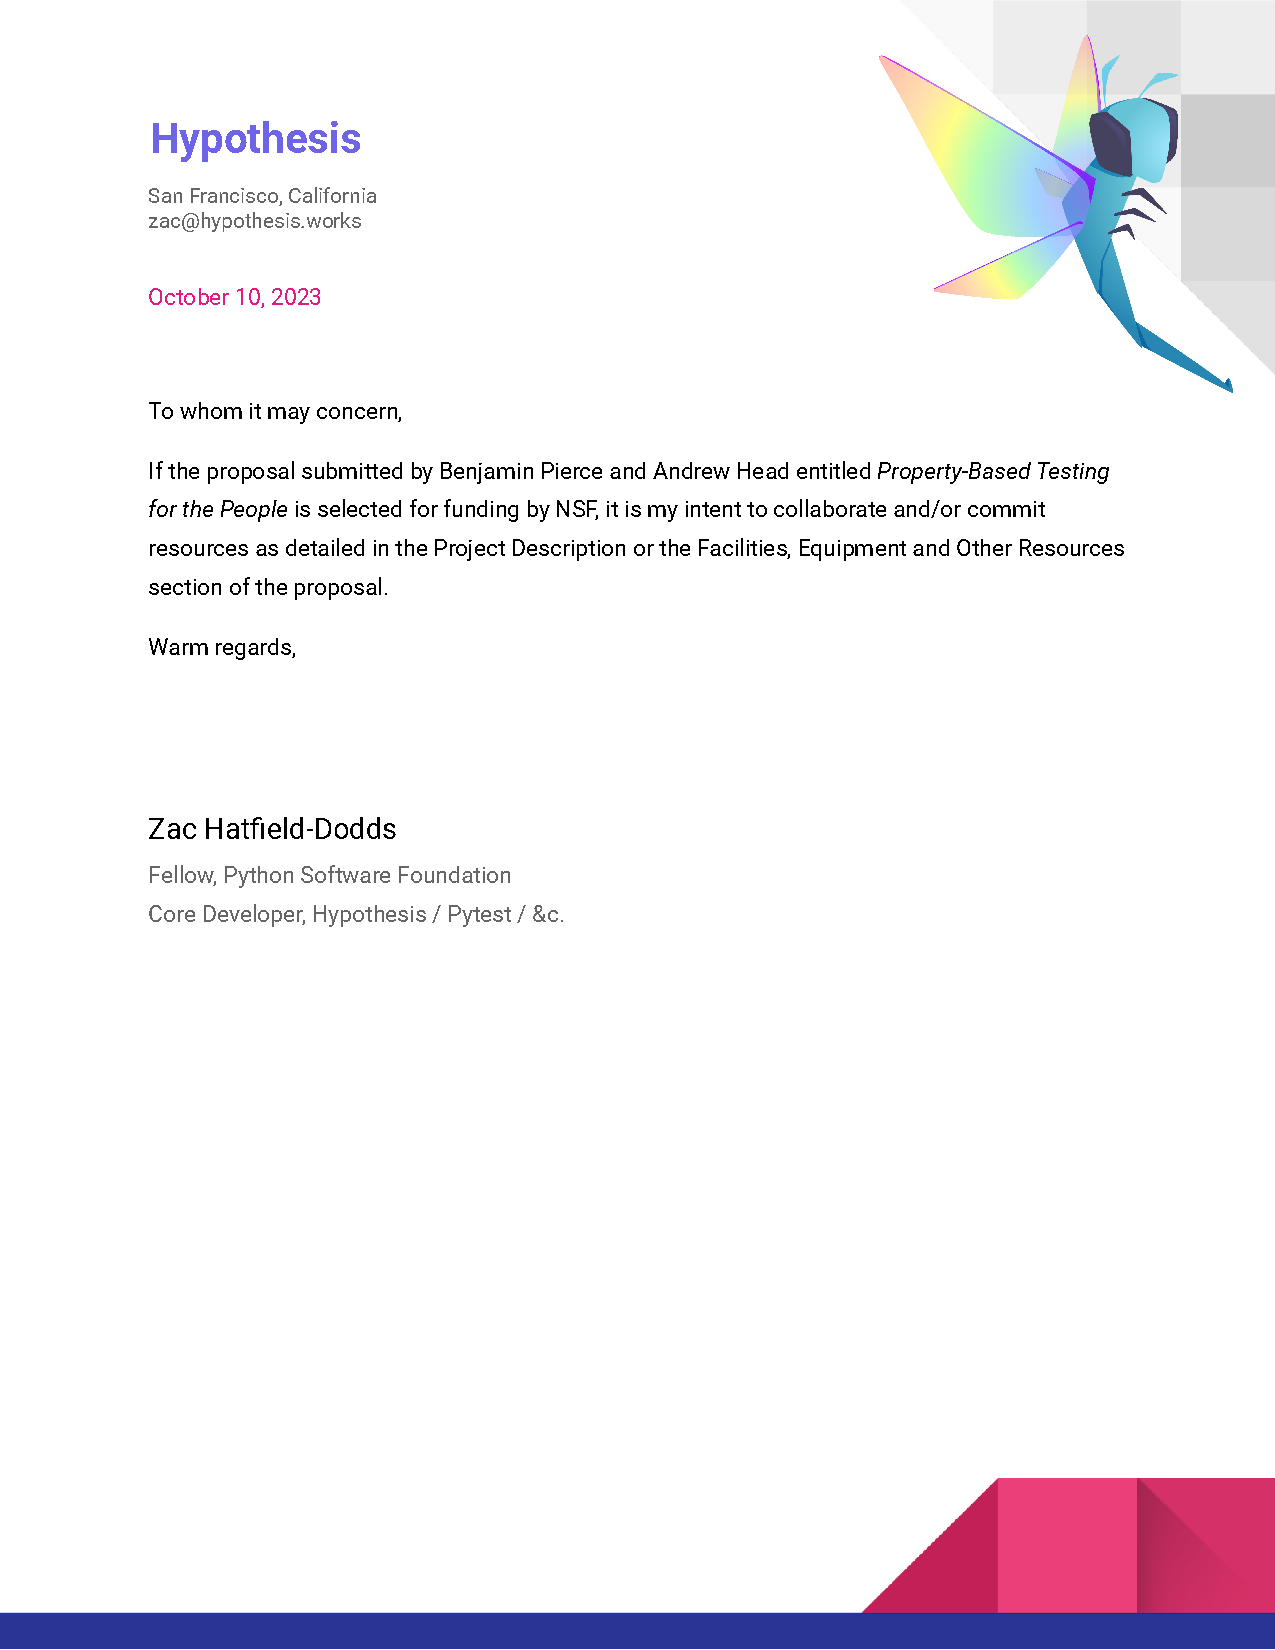
\includepdf[pages=-]{assets/Zac-letter.pdf}

\end{document}
